\documentclass{report}
\usepackage[left=3cm,right=3cm,top=2cm,bottom=2cm]{geometry} % page settings
\usepackage{amsmath,amssymb,amsthm,float,graphicx,hhline,listings,enumitem,hyperref} % provides many mathematical environments & tools
\hypersetup{
	colorlinks=true,
	linkcolor=blue,
	filecolor=magenta,      
	urlcolor=cyan,
}

\setlength{\parindent}{0mm}

%https://tex.stackexchange.com/questions/45817/theorem-definition-lemma-problem-numbering
\theoremstyle{plain}
\newtheorem{thm}{Theorem}[chapter] % reset theorem numbering for each chapter
\theoremstyle{definition}
\newtheorem{defn}[thm]{Definition} % definition numbers are dependent on theorem numbers
\newtheorem{exmp}[thm]{Example} % same for example numbers

\renewcommand{\labelitemii}{$\star$}

\begin{document}

\title{CQF: Final Project}
\author{Joseph Dwonczyk }
\date{\today}
\maketitle

\part{CVA Valuation}
\chapter{Introduction to CVA}title
In this section, I calculate the credit valuation adjustment (CVA) taken by a Counterparty A when they enter a vanilla interest rate swap with a Counterparty B in which Counterparty A pays fixed payments and receives floating payments. In this project, I will use a European bank as an example Counterparty B as there is much more data available on the probabilty of default of major European banks. 

\chapter{Data Collection}
For this part of the project I require the following data:
\begin{itemize}
	\item Discount Curves for discounting simulated future cash flows in the Interest Rate swap:
	\begin{itemize}
		\item LIBOR
		\item SONIA
	\end{itemize}
	\item Default Rates for Counterparty B:
	\begin{itemize}
		\item Credit Spreads for Tenors out to 5 years to cover the lifetime of the swap. 
	\end{itemize}	

\end{itemize}

To fetch this data, I have used the Bloomberg terminal of a colleague.

For fetching the Discount rates, I fetch the spot rates for LIBOR and SONIA and bootstrap the implied Discount rates as follows. I first grab the discount factors for the observed tenors:

\begin{align*}
	DF_{i}(0,\tau) = {\Big(\frac{1}{1+i}\Big)}^{t}
\end{align*}

I next interpolate the discount factors so that we can look at the exposure of Counterparty A to Counterparty B over smaller windows in the future. We will use months (1/12 years) as the timestep and review later if there is any evidence that more timesteps are required. I use a log-linear interpolation as the discount factor is the inverse of the rate that we are observing in the market. i.e.

\begin{align*}
	logDF(0,\tau) = \frac{\tau - \tau_i}{\tau_{i+1} - \tau_{i}}logDF(0,\tau_{i+1}) + \frac{\tau_{i+1} - \tau}{\tau_{i+1} - \tau_{i}}logDF(0,\tau_{i})
\end{align*}

For fetching the default probabilities of Counterparty B, I pull the Credit Default Swap Spreads for the Tenors of 1 out to 5 years inclusive. I then make the assumption that the market prices of these values are sufficiently liquid to infer the Markets view on \textbf{the price of the probability of default of Counterparty B}. I then use these values as a proxy for the probability of default of Counterparty B until the respective tenor. For example, the 5 year CDS can be used to derive a proxy for the probability that Counterparty B defaults between now and 5 years time.
I then again interpolate the default probabilities to monthly periods using a linear interpolation for the same reason as above.



\pagebreak

\chapter{Forward-Rate Simulation in the Heath-Jarrow-Morton Family}

I this project, I have decided to model the forward rates in the HJM family of models as follows: 

\begin{align*}
	%HJM drift + vol formula.
\end{align*}

This can be seen by starting with the relationship between the price of a Bond at time $t$ today, $Z(t,T)$ and the instantaneous forward rate $f(t,T)$ out to time $T$ as seed from time $t$:
\begin{align*}
	Z(t,T) = e^{}-\int_t^Tf(t,s)ds = -\frac{\partial}{\partial T}logZ(t,T)
\end{align*}
Under the HJM framwork we then use the Bond Pricing Equation to give us: 
\begin{equation}
	df(t,T) = \frac{\partial}{\partial T}\Big{[}\frac{1}{2}\sigma^2(t,T) - \mu(t,T) \Big{]} dt - \frac{\partial}{\partial T} \sigma(t,T)dW_t
\label{HJM:Update}
\end{equation}
where $\mu$ defines the drift function for the bond price and $\sigma$ the volatility of the bond price. We next consider the BPE under the risk neutral measure which would give us the same as above but with $\mu^{\mathbf{Q}}(t,T) = r(t)$ and $dW_t^{\mathbf{Q}}$. I notice that as $r(t)$ is not $T$-dependent, the partial derivative wrt $T$ is by definition 0. We apply the change of measure under the result of Girsanov's thm.

We are then able to setup a Hedged portfolio using a bond of different maturity. In doing so we discover that we are able to separate the Hedged portfolio into 2 different parts; the first which depends on the first bonds maturity and the second likewise. Which tells us at the Market price of risk, $\lambda(t)$, must be independent of maturity. Thus after some simplification, we have:
\begin{equation}
	df(t,T) = \sigma(t,T)\frac{\partial}{\partial T}\sigma(t,T)dt - \frac{\partial }{\partial T}\sigma(t,T) dW_t^{\mathbf{Q}}
\label{HJM:riskfree}
\end{equation}
With this in mind, I fetch historical Libor spot rates for the last 3 years so that there are sufficient data points. I fetch this data for each tenor: 1 month, 6 months, 12 months out to 50 years. I then bootstap the forward rates from the spot rates for each historical date. From the historical forward rates, I can now conduct a Principal Component Analysis on the different rates out to 50 years to conclude which rates are historically the most significant. I will then simulate these significant rates in order to simulate the outcome of the vanilla interest rate swap. The Monte carlo simulation would be too slow if we chose to evolve all of the rates as it would become a very high dimensional problem with each forward rate adding a new dimension.

To conduct the principal component analysis of the forward rates, I first calculate the matrix of absolute differences (day-by-day) in forward rates in order to then calculate the covariance matrix for the forward rates. I then calculate the eigenvalues and respective eigenvalues for the covariance matrix as below:


\begin{center}
 \begin{tabular}{|l|l|l|l|l|l|l|l|l|l|l|l|l|l|l|l|l|l|l|l|l|l|l|l|l|l|c|c|c|c|c|c|c|c|c|c|c|c|c|c|c|c|c|c|c|c|c|c|c|c|c|c|}
\hline
& \textbf{0} & \textbf{1} & \textbf{2} & \textbf{3} & \textbf{4} & \textbf{5} & \textbf{6} & \textbf{7} & \textbf{8} & \textbf{9} & \textbf{10} & \textbf{11} & \textbf{12} & \textbf{13} & \textbf{14} & \textbf{15} & \textbf{16} & \textbf{17} & \textbf{18} & \textbf{19} & \textbf{20} & \textbf{21} & \textbf{22} & \textbf{23} & \textbf{24} & \textbf{25}\\\hhline{|=|=|=|=|=|=|=|=|=|=|=|=|=|=|=|=|=|=|=|=|=|=|=|=|=|=|=|}
\textbf{0} & 1.0 & 2.5479834212e-06 & 3.26647738456e-06 & 2.29331392091e-05 & -3.60862585462e-06 & -1.32026977123e-06 & 1.00818266744e-05 & 2.2148730266e-05 & 1.19383372506e-05 & 2.52316935023e-05 & 1.05765572324e-05 & 1.01385544238e-05 & 7.18211921494e-06 & 3.18094384313e-06 & 4.29203016265e-06 & 6.46842241308e-06 & 4.75281485517e-06 & 2.01341647183e-05 & 9.49095865681e-06 & 3.74920468535e-07 & -9.74278493378e-06 & -7.97986981484e-07 & -1.45246688963e-05 & 7.52077449756e-06 & 9.16448315967e-06 & 6.34434048042e-06\\
\textbf{1} & 2.5479834212e-06 & 1.0 & -5.44517950652e-08 & -5.91168281189e-05 & 2.26947689793e-05 & 2.83177431241e-05 & 4.97124617692e-05 & -2.82866240003e-05 & 4.61319589783e-05 & 4.29989571905e-05 & 2.35182991259e-05 & 1.8492492678e-05 & 1.47635282991e-05 & 1.12097899388e-05 & 6.24840158264e-06 & 1.12710111731e-05 & 9.70351293336e-06 & 2.86751897321e-05 & 1.76255734581e-05 & 3.37183040588e-06 & -1.00756519112e-05 & 8.45714937594e-07 & -1.45166579959e-05 & 1.85297948185e-05 & 1.27739276181e-05 & 1.03143285393e-05\\
\textbf{2} & 3.26647738456e-06 & -5.44517950652e-08 & 1.0 & 0.000171578302069 & -3.25578910033e-05 & -3.24196198103e-05 & -2.45824600446e-05 & 0.000219743415952 & 5.03510705643e-05 & 8.66693856812e-05 & 7.11575552309e-05 & 7.06599913062e-05 & 6.18264553988e-05 & 5.37290897304e-05 & 4.10532780364e-05 & 5.72466167378e-05 & 5.91613501244e-05 & 6.76206239852e-05 & 8.2907630706e-05 & 4.75075935483e-05 & 3.79972528656e-05 & 3.26054765205e-05 & 1.79831374843e-05 & 4.04583332064e-05 & 3.29017680324e-05 & 3.2287019978e-05\\
\textbf{3} & 2.29331392091e-05 & -5.91168281189e-05 & 0.000171578302069 & 1.0 & -0.000873518055955 & -0.000945510801984 & -0.00103519482214 & 0.00235641517881 & -0.000651597802177 & 7.97753631638e-05 & 2.81091444219e-05 & 4.29719738392e-05 & 6.51366373902e-07 & -9.3569807032e-05 & -2.3762719505e-05 & 2.64717658404e-05 & 3.08850143083e-07 & 2.91627788768e-05 & 2.98240353677e-05 & -1.44767380782e-05 & -4.73653426559e-05 & -3.2473694431e-06 & -7.21096279405e-05 & -4.39152919981e-06 & 3.2967333407e-06 & -1.0304934076e-05\\
\textbf{4} & -3.60862585462e-06 & 2.26947689793e-05 & -3.25578910033e-05 & -0.000873518055955 & 1.0 & 0.000246162870129 & 0.000356696623934 & -0.000625882887944 & 0.000391703865431 & 8.60652306779e-05 & 8.54576009618e-05 & 8.96471920099e-05 & 7.5455438304e-05 & 2.97292693313e-05 & 3.53115398284e-05 & 4.96030842502e-05 & 5.22401026608e-05 & 6.33553978083e-05 & 7.22569418738e-05 & 4.78854110934e-05 & 3.87478508083e-05 & 2.72643417549e-05 & 3.75032887559e-05 & 6.00574923196e-05 & 4.56628924553e-05 & 4.12952212691e-05\\
\textbf{5} & -1.32026977123e-06 & 2.83177431241e-05 & -3.24196198103e-05 & -0.000945510801984 & 0.000246162870129 & 1.0 & 0.000396143141887 & -0.00070533791788 & 0.000357085126393 & 0.000144142994965 & 0.000108640616017 & 8.69126896997e-05 & 8.99140552632e-05 & 0.000116775057765 & 4.75419498808e-05 & 7.06830822346e-05 & 7.41109301725e-05 & 0.000102830647535 & 0.000101450496714 & 6.65839408428e-05 & 4.9735310483e-05 & 4.14489396834e-05 & 2.09456594156e-05 & 8.35724773313e-05 & 4.50345429094e-05 & 5.11215504108e-05\\
\textbf{6} & 1.00818266744e-05 & 4.97124617692e-05 & -2.45824600446e-05 & -0.00103519482214 & 0.000356696623934 & 0.000396143141887 & 1.0 & -0.00048832938192 & 0.00135312252493 & 0.000917420509376 & 0.000548164781432 & 0.000473705191846 & 0.000291629558944 & -4.91689879981e-05 & -6.44559551101e-05 & 0.000188125860253 & 0.000161187087808 & 0.000484330942852 & 0.000341236452157 & -2.26467679602e-05 & -0.000244988625865 & -5.83712737799e-05 & -0.000357315020622 & 0.000304247171232 & 0.000134549322385 & 7.91521476636e-05\\
\textbf{7} & 2.2148730266e-05 & -2.82866240003e-05 & 0.000219743415952 & 0.00235641517881 & -0.000625882887944 & -0.00070533791788 & -0.00048832938192 & 1.0 & 0.00056677801 & 0.000967658962074 & 0.00057499449873 & 0.000469121604009 & 0.000212440316235 & -0.00017243768423 & -0.000280568835641 & 0.000152288489628 & 9.5244018062e-05 & 0.000301800782639 & 0.000336595578746 & -4.34473494443e-06 & -0.000229665739009 & -0.000104784444384 & -0.000248754671383 & 0.000479724779021 & 5.00201242676e-05 & 4.13365115363e-05\\
\textbf{8} & 1.19383372506e-05 & 4.61319589783e-05 & 5.03510705643e-05 & -0.000651597802177 & 0.000391703865431 & 0.000357085126393 & 0.00135312252493 & 0.00056677801 & 1.0 & 0.00240214530845 & 0.00162561811485 & 0.00229495945346 & 0.000757459438363 & -0.00262403746995 & -0.00242298605726 & 0.000190377089663 & 0.000168973235234 & 0.000426017060988 & 0.000342568154463 & 1.9482967972e-05 & -0.000169446805007 & -3.74609603379e-05 & -0.000258573209241 & 0.000318581108491 & 0.000122879590923 & 8.08091610647e-05\\
\textbf{9} & 2.52316935023e-05 & 4.29989571905e-05 & 8.66693856812e-05 & 7.97753631638e-05 & 8.60652306779e-05 & 0.000144142994965 & 0.000917420509376 & 0.000967658962074 & 0.00240214530845 & 1.0 & 0.00132310356882 & 0.0011092733711 & 0.000672161993912 & -0.000168293158937 & 9.83205304523e-05 & 0.000408979737837 & 0.000215876115802 & 0.000822382951678 & 0.000721086639674 & -0.000370413017135 & -0.000511620375955 & -0.000164012867097 & -0.000769499606379 & 0.000716798660633 & 0.000211042896807 & 9.85891392068e-05\\
\textbf{10} & 1.05765572324e-05 & 2.35182991259e-05 & 7.11575552309e-05 & 2.81091444219e-05 & 8.54576009618e-05 & 0.000108640616017 & 0.000548164781432 & 0.00057499449873 & 0.00162561811485 & 0.00132310356882 & 1.0 & 0.000846838440248 & 0.000559665331292 & -2.32702716803e-05 & 0.000192670688 & 0.000430230326549 & 0.000358967774126 & 0.000540697554928 & 0.000488059849071 & -0.000113604322234 & -0.000199585824254 & 0.000102410239262 & -0.000296307323393 & 0.000300811280622 & 9.70753270574e-05 & 7.40487653654e-05\\
\textbf{11} & 1.01385544238e-05 & 1.8492492678e-05 & 7.06599913062e-05 & 4.29719738392e-05 & 8.96471920099e-05 & 8.69126896997e-05 & 0.000473705191846 & 0.000469121604009 & 0.00229495945346 & 0.0011092733711 & 0.000846838440248 & 1.0 & 0.000550345082022 & -0.000441630357145 & -0.000195344812247 & 0.000398028642391 & 0.000364224614224 & 0.00047584027722 & 0.000444952076998 & 6.10096799159e-05 & -1.28296118962e-06 & 0.000170162769655 & -0.000126210095688 & 7.68126328129e-05 & 0.000107833980392 & 7.68485918509e-05\\
\textbf{12} & 7.18211921494e-06 & 1.47635282991e-05 & 6.18264553988e-05 & 6.51366373902e-07 & 7.5455438304e-05 & 8.99140552632e-05 & 0.000291629558944 & 0.000212440316235 & 0.000757459438363 & 0.000672161993912 & 0.000559665331292 & 0.000550345082022 & 1.0 & 0.000257058222818 & 0.00054037306478 & 0.000487885139364 & 0.000459905388112 & 0.000587479338649 & 0.000612707351999 & 0.000166261905554 & 0.000177908973714 & 0.000204622421511 & -6.21040169135e-05 & -6.34228317459e-06 & 0.00011922558317 & 7.87096278551e-05\\
\textbf{13} & 3.18094384313e-06 & 1.12097899388e-05 & 5.37290897304e-05 & -9.3569807032e-05 & 2.97292693313e-05 & 0.000116775057765 & -4.91689879981e-05 & -0.00017243768423 & -0.00262403746995 & -0.000168293158937 & -2.32702716803e-05 & -0.000441630357145 & 0.000257058222818 & 1.0 & 0.00115885933558 & 0.000594987048984 & 0.000566401598651 & 0.000705253053969 & 0.000786643250029 & 0.000227613614462 & 0.000251001247288 & 0.000254281139112 & -4.98442436121e-05 & -5.40058992021e-05 & 0.000123565443846 & 7.71982045345e-05\\
\textbf{14} & 4.29203016265e-06 & 6.24840158264e-06 & 4.10532780364e-05 & -2.3762719505e-05 & 3.53115398284e-05 & 4.75419498808e-05 & -6.44559551101e-05 & -0.000280568835641 & -0.00242298605726 & 9.83205304523e-05 & 0.000192670688 & -0.000195344812247 & 0.00054037306478 & 0.00115885933558 & 1.0 & 0.000671254047864 & 0.000518736232376 & 0.000579091601869 & 0.000777557690673 & -0.000109046308329 & 0.000347728272483 & 0.000279092442584 & -6.73943331489e-06 & -0.000136414494376 & 0.000111038400661 & 5.82013352399e-05\\
\textbf{15} & 6.46842241308e-06 & 1.12710111731e-05 & 5.72466167378e-05 & 2.64717658404e-05 & 4.96030842502e-05 & 7.06830822346e-05 & 0.000188125860253 & 0.000152288489628 & 0.000190377089663 & 0.000408979737837 & 0.000430230326549 & 0.000398028642391 & 0.000487885139364 & 0.000594987048984 & 0.000671254047864 & 1.0 & 0.00067443310291 & 0.000802746188514 & 0.000788824326105 & 0.000466909884399 & 0.000290907337194 & 0.000357586030079 & -2.65792265113e-05 & -0.000126095415222 & 0.000100392919403 & 5.12034339805e-05\\
\textbf{16} & 4.75281485517e-06 & 9.70351293336e-06 & 5.91613501244e-05 & 3.08850143083e-07 & 5.22401026608e-05 & 7.41109301725e-05 & 0.000161187087808 & 9.5244018062e-05 & 0.000168973235234 & 0.000215876115802 & 0.000358967774126 & 0.000364224614224 & 0.000459905388112 & 0.000566401598651 & 0.000518736232376 & 0.00067443310291 & 1.0 & 0.000868907470207 & 0.00074716951088 & 0.000738039692906 & 0.000325231137685 & 0.000367137494683 & 1.90980121393e-05 & -0.000181387676137 & 9.50797913864e-05 & 6.65504933836e-05\\
\textbf{17} & 2.01341647183e-05 & 2.86751897321e-05 & 6.76206239852e-05 & 2.91627788768e-05 & 6.33553978083e-05 & 0.000102830647535 & 0.000484330942852 & 0.000301800782639 & 0.000426017060988 & 0.000822382951678 & 0.000540697554928 & 0.00047584027722 & 0.000587479338649 & 0.000705253053969 & 0.000579091601869 & 0.000802746188514 & 0.000868907470207 & 1.0 & 0.00155360701346 & 0.00091279964023 & 9.23102284824e-05 & 0.000181606371741 & -0.000710435767731 & -6.34074946212e-05 & 0.000241459544446 & 2.55482392781e-05\\
\textbf{18} & 9.49095865681e-06 & 1.76255734581e-05 & 8.2907630706e-05 & 2.98240353677e-05 & 7.22569418738e-05 & 0.000101450496714 & 0.000341236452157 & 0.000336595578746 & 0.000342568154463 & 0.000721086639674 & 0.000488059849071 & 0.000444952076998 & 0.000612707351999 & 0.000786643250029 & 0.000777557690673 & 0.000788824326105 & 0.00074716951088 & 0.00155360701346 & 1.0 & 0.00108243684505 & 0.000588871639725 & 0.00011824963598 & -0.000378519134596 & -1.93557596004e-06 & 0.000110530851612 & 2.95149748622e-06\\
\textbf{19} & 3.74920468535e-07 & 3.37183040588e-06 & 4.75075935483e-05 & -1.44767380782e-05 & 4.78854110934e-05 & 6.65839408428e-05 & -2.26467679602e-05 & -4.34473494443e-06 & 1.9482967972e-05 & -0.000370413017135 & -0.000113604322234 & 6.10096799159e-05 & 0.000166261905554 & 0.000227613614462 & -0.000109046308329 & 0.000466909884399 & 0.000738039692906 & 0.00091279964023 & 0.00108243684505 & 1.0 & 0.000678909099363 & 0.000287262335912 & 0.000147768231828 & -0.000216889895579 & 4.56716298275e-05 & 1.44333900276e-05\\
\textbf{20} & -9.74278493378e-06 & -1.00756519112e-05 & 3.79972528656e-05 & -4.73653426559e-05 & 3.87478508083e-05 & 4.9735310483e-05 & -0.000244988625865 & -0.000229665739009 & -0.000169446805007 & -0.000511620375955 & -0.000199585824254 & -1.28296118962e-06 & 0.000177908973714 & 0.000251001247288 & 0.000347728272483 & 0.000290907337194 & 0.000325231137685 & 9.23102284824e-05 & 0.000588871639725 & 0.000678909099363 & 1.0 & 0.000244232001535 & 0.000597076148063 & -0.000269633265177 & -2.94452229654e-05 & 4.49246129919e-05\\
\textbf{21} & -7.97986981484e-07 & 8.45714937594e-07 & 3.26054765205e-05 & -3.2473694431e-06 & 2.72643417549e-05 & 4.14489396834e-05 & -5.83712737799e-05 & -0.000104784444384 & -3.74609603379e-05 & -0.000164012867097 & 0.000102410239262 & 0.000170162769655 & 0.000204622421511 & 0.000254281139112 & 0.000279092442584 & 0.000357586030079 & 0.000367137494683 & 0.000181606371741 & 0.00011824963598 & 0.000287262335912 & 0.000244232001535 & 1.0 & 0.000201725995945 & -0.000244624776866 & 9.56320627363e-05 & 7.80366515971e-05\\
\textbf{22} & -1.45246688963e-05 & -1.45166579959e-05 & 1.79831374843e-05 & -7.21096279405e-05 & 3.75032887559e-05 & 2.09456594156e-05 & -0.000357315020622 & -0.000248754671383 & -0.000258573209241 & -0.000769499606379 & -0.000296307323393 & -0.000126210095688 & -6.21040169135e-05 & -4.98442436121e-05 & -6.73943331489e-06 & -2.65792265113e-05 & 1.90980121393e-05 & -0.000710435767731 & -0.000378519134596 & 0.000147768231828 & 0.000597076148063 & 0.000201725995945 & 1.0 & -0.000151623293577 & -4.45527071902e-05 & 0.000148149152768\\
\textbf{23} & 7.52077449756e-06 & 1.85297948185e-05 & 4.04583332064e-05 & -4.39152919981e-06 & 6.00574923196e-05 & 8.35724773313e-05 & 0.000304247171232 & 0.000479724779021 & 0.000318581108491 & 0.000716798660633 & 0.000300811280622 & 7.68126328129e-05 & -6.34228317459e-06 & -5.40058992021e-05 & -0.000136414494376 & -0.000126095415222 & -0.000181387676137 & -6.34074946212e-05 & -1.93557596004e-06 & -0.000216889895579 & -0.000269633265177 & -0.000244624776866 & -0.000151623293577 & 1.0 & 0.000231218657062 & 0.000196840205256\\
\textbf{24} & 9.16448315967e-06 & 1.27739276181e-05 & 3.29017680324e-05 & 3.2967333407e-06 & 4.56628924553e-05 & 4.50345429094e-05 & 0.000134549322385 & 5.00201242676e-05 & 0.000122879590923 & 0.000211042896807 & 9.70753270574e-05 & 0.000107833980392 & 0.00011922558317 & 0.000123565443846 & 0.000111038400661 & 0.000100392919403 & 9.50797913864e-05 & 0.000241459544446 & 0.000110530851612 & 4.56716298275e-05 & -2.94452229654e-05 & 9.56320627363e-05 & -4.45527071902e-05 & 0.000231218657062 & 1.0 & 0.000170051077602\\
\textbf{25} & 6.34434048042e-06 & 1.03143285393e-05 & 3.2287019978e-05 & -1.0304934076e-05 & 4.12952212691e-05 & 5.11215504108e-05 & 7.91521476636e-05 & 4.13365115363e-05 & 8.08091610647e-05 & 9.85891392068e-05 & 7.40487653654e-05 & 7.68485918509e-05 & 7.87096278551e-05 & 7.71982045345e-05 & 5.82013352399e-05 & 5.12034339805e-05 & 6.65504933836e-05 & 2.55482392781e-05 & 2.95149748622e-06 & 1.44333900276e-05 & 4.49246129919e-05 & 7.80366515971e-05 & 0.000148149152768 & 0.000196840205256 & 0.000170051077602 & 1.0\\
\hline
\end{tabular}
\end{center}

\section{Eigen-Values}
\begin{center}
 \begin{tabular}{|l|l|l|l|l|l|l|l|l|l|l|l|l|l|l|l|l|l|l|l|l|l|l|l|l|l|c|c|c|c|c|c|c|c|c|c|c|c|c|c|c|c|c|c|c|c|c|c|c|c|c|c|}
\hline
& \textbf{0} & \textbf{1} & \textbf{2} & \textbf{3} & \textbf{4} & \textbf{5} & \textbf{6} & \textbf{7} & \textbf{8} & \textbf{9} & \textbf{10} & \textbf{11} & \textbf{12} & \textbf{13} & \textbf{14} & \textbf{15} & \textbf{16} & \textbf{17} & \textbf{18} & \textbf{19} & \textbf{20} & \textbf{21} & \textbf{22} & \textbf{23} & \textbf{24} & \textbf{25}\\\hhline{|=|=|=|=|=|=|=|=|=|=|=|=|=|=|=|=|=|=|=|=|=|=|=|=|=|=|=|}
\textbf{Eigen values} & 1.00756256558 & 1.00545869247 & 1.00374441381 & 1.00178751973 & 1.0006608268 & 1.00033096681 & 1.00000422781 & 0.999995723396 & 0.999991269471 & 0.999951155789 & 0.999796459062 & 0.999755420798 & 0.999665068993 & 0.99946041729 & 0.999437581614 & 0.999381561981 & 0.99925630034 & 0.999084929437 & 0.998998830927 & 0.998912653931 & 0.998737688183 & 0.998589739523 & 0.998347247124 & 0.998178282873 & 0.997430239198 & 0.995480217061\\
\hline
\end{tabular}
\end{center}


%Make landscape and place in CVA Section appendices for all big tables like this.
\section{Eigen-vectors}

\begin{center}
 \begin{tabular}{|l|l|l|l|l|l|l|l|l|l|l|l|l|l|l|l|l|l|l|l|l|l|l|l|l|l|c|c|c|c|c|c|c|c|c|c|c|c|c|c|c|c|c|c|c|c|c|c|c|c|c|c|}
\hline
& \textbf{0} & \textbf{1} & \textbf{2} & \textbf{3} & \textbf{4} & \textbf{5} & \textbf{6} & \textbf{7} & \textbf{8} & \textbf{9} & \textbf{10} & \textbf{11} & \textbf{12} & \textbf{13} & \textbf{14} & \textbf{15} & \textbf{16} & \textbf{17} & \textbf{18} & \textbf{19} & \textbf{20} & \textbf{21} & \textbf{22} & \textbf{23} & \textbf{24} & \textbf{25}\\\hhline{|=|=|=|=|=|=|=|=|=|=|=|=|=|=|=|=|=|=|=|=|=|=|=|=|=|=|=|}
\textbf{0} & -0.00531884181795 & -0.00293574987334 & 0.00772743976615 & 0.00924002346893 & 0.0049586285041 & -0.0206055832547 & 0.790310174202 & -0.256541662673 & 0.549276716695 & 0.0832680364461 & -0.0127617199693 & 0.000327519972466 & 0.00610201699353 & 0.00238376957367 & 0.00453471341697 & 0.001036228011 & 0.00107725440003 & 0.00188561148867 & -0.00403200369894 & -0.00755459065223 & 0.00222467401768 & -0.00141005536316 & 0.00259946916699 & 0.001639450155 & -0.00212856509312 & 0.000258956707667\\
\textbf{1} & -0.0113099981815 & -0.00386526369613 & -0.0210052728466 & 0.0189827928331 & 0.000577319079393 & -0.0393966700846 & 0.323965790876 & 0.941622048024 & -0.0376022821698 & 0.0621322664327 & -0.0167095772262 & 0.00804673543384 & -0.00561696058311 & -0.00254595100654 & -0.0125813523014 & -0.00236955882825 & 0.000171992154312 & 0.00303418544253 & -0.00245428389995 & 0.00178021904916 & -0.00157050055619 & 0.00389066901832 & -0.000348159633041 & 0.00560734936003 & 0.00242566038088 & 0.00187155184036\\
\textbf{2} & -0.0229776032602 & -0.0287726367495 & 0.0687886905288 & -0.0208278341729 & -0.0946648919415 & -0.13465754412 & -0.24433044911 & 0.152551625634 & 0.534138112753 & -0.762627725711 & 0.0508726558719 & 0.0167122107361 & -0.0884105880787 & 0.0193886888232 & 0.0471672460023 & 0.000649060246622 & -0.0146196107214 & 0.023668015972 & -0.0217554141723 & -0.041301337838 & -0.00793812439168 & -0.0112463078378 & -0.000120008236659 & 0.00264369634526 & 0.00713714691989 & 0.00501569116705\\
\textbf{3} & 0.0288686707545 & -0.0258830431473 & 0.608596900875 & -0.0719457459258 & -0.0211774345217 & -0.00562824065444 & 0.0149235214193 & 0.00273571559258 & -0.021217649056 & 0.0153388066933 & -0.0078535867704 & 0.00814837039995 & 0.0238865241261 & -0.0421779367125 & -0.134978281833 & -0.0152254671852 & 0.00310877524751 & -0.0508708337213 & 0.0547064910048 & 0.267072314892 & -0.0529891430414 & 0.169846349317 & -0.10246992936 & 0.127286227231 & 0.672683011557 & -0.113260900871\\
\textbf{4} & -0.0498471523378 & -0.00359445651822 & -0.292863576596 & 0.0316851634439 & -0.0446904593942 & -0.0664768315553 & -0.0562903844114 & -0.00341537921421 & 0.0809721254769 & -0.00467136400981 & -0.214452617682 & 0.722778717898 & 0.240492765386 & -0.131432988353 & -0.440448900984 & -0.0433417275542 & 0.000545710009265 & -0.0398189524266 & 0.032957800353 & 0.205062472662 & -0.0220190755193 & 0.0716912293406 & -0.0321489864073 & 0.0339652832975 & 0.0416888058145 & 0.0299647107778\\
\textbf{5} & -0.0525070835336 & -0.0208195367295 & -0.31612903875 & 0.0592707030281 & -0.0388549794042 & -0.0851824330213 & -0.0527487681576 & 0.00783346484906 & 0.0912544245081 & 0.00222134978342 & 0.126909269064 & -0.632439594753 & 0.104858136782 & -0.14926989818 & -0.585426275429 & -0.0547225633843 & -0.0158871208456 & -0.0369926659782 & 0.039715374964 & 0.233034065326 & -0.0678776510594 & 0.0973433417152 & -0.0406304079725 & 0.0592157689578 & 0.0315134787546 & 0.0244849033595\\
\textbf{6} & -0.240290758075 & -0.00372587386789 & -0.289096883055 & 0.186837727662 & 0.0689097502534 & -0.0459087611128 & 0.0023865572855 & -0.00841898608007 & 0.00044074326595 & -0.028657536729 & 0.0622956759797 & -0.00696315391694 & -0.0208839569186 & 0.143969802475 & 0.50699434457 & 0.0603651732678 & 0.00728398853368 & -0.191708972458 & 0.134814721303 & 0.569703809532 & -0.0272935674002 & 0.327244948854 & -0.0850958609206 & 0.160001021091 & 0.0433062003641 & 0.0901828839142\\
\textbf{7} & -0.154601661729 & -0.00608836690884 & 0.569306766613 & -0.00627378074096 & -0.0177832187791 & -0.0817984519098 & -0.0269448923686 & 0.0144075716128 & 0.0277509723691 & 0.0505940082117 & -0.0088982242792 & 0.00609293845198 & 0.123061381981 & -0.0343679322917 & -0.138311270751 & -0.000427542505364 & -0.00261442792098 & -0.103941405112 & 0.0593910273234 & 0.313742895735 & -0.0035399005858 & 0.0796650160635 & 0.0104426725716 & 0.00620493520572 & -0.696103960888 & 0.0350624655936\\
\textbf{8} & -0.533205909577 & 0.266469320033 & -0.0801093955313 & -0.206371781104 & 0.00817851176261 & 0.0100027652236 & 0.00524764330649 & -0.00265742866663 & -0.00706830001662 & -0.00453158991624 & -0.00566517415006 & -0.00313883165906 & -0.0235184062881 & 0.00242863518231 & 0.00342048059398 & -0.0125872494739 & -0.0240422473004 & 0.0162733627613 & -0.0395234337515 & 0.00573313081919 & -0.0183061710341 & -0.107680584789 & 0.0363268581256 & -0.00838703183102 & -0.0079323799852 & -0.760798686807\\
\textbf{9} & -0.422074949057 & -0.0154042868625 & 0.080428674857 & 0.259243688597 & -0.0533729361132 & 0.0174378185349 & -0.0392767910637 & 0.00752111473129 & 0.0450230195349 & 0.0572454775337 & -0.0122806522267 & -0.016941987283 & 0.0261615425211 & -0.0233590206994 & 0.0114636495848 & -0.0767941193924 & 0.0570355304767 & 0.000351884616314 & 0.0403758378356 & 0.0892169177566 & -0.11893784943 & -0.233220152104 & 0.283430991169 & -0.678945176741 & 0.196542583052 & 0.262444388996\\
\textbf{10} & -0.318902578204 & -0.0581448755073 & 0.0441665471977 & 0.129099835096 & -0.216549385336 & 0.141845516859 & -0.0377040879184 & 0.0103001319814 & 0.0434863468702 & 0.0548842259013 & 0.00941571304226 & -0.0172597102347 & 0.118983974788 & 0.104376487121 & -0.0393064163355 & -0.0947817985277 & 0.37471356715 & -0.368005464164 & -0.548345685123 & -0.26962013229 & 0.151914722098 & 0.157870131164 & -0.127372322995 & 0.186366468787 & 0.0349754945693 & 0.132266677951\\
\textbf{11} & -0.35275591155 & 0.0158328719008 & 0.0146575874586 & -0.145787032985 & -0.175767991229 & 0.139479970648 & 0.0135663833826 & -0.00268841275769 & -0.0148765706467 & -0.000619460561612 & -0.0241422844881 & -0.00201720232995 & -0.0757542160103 & 0.057213682574 & -0.0717917268992 & -0.142760640325 & 0.123875616945 & 0.258765231362 & 0.615332519494 & -0.286537156638 & 0.276504751469 & 0.294695202029 & -0.0962781661748 & 0.0925300237042 & 0.00330378182782 & 0.209197455231\\
\textbf{12} & -0.18618569801 & -0.181663690213 & -0.0041869715873 & -0.00435259478668 & -0.274464336464 & 0.180325722327 & -0.0524171072888 & 0.0130245410408 & 0.0718278371956 & 0.115294732765 & -0.138202339092 & 0.00424900188264 & -0.364453763294 & -0.401129417335 & -0.00751211531815 & 0.548855170092 & -0.383784584244 & -0.0287271097996 & -0.114796064435 & 0.0131488328597 & 0.130736271483 & 0.0140933711263 & -0.0214769467519 & 0.0591198830444 & 0.00423389309979 & 0.0787389444384\\
\textbf{13} & 0.177765878759 & -0.412385499447 & -0.0112003310842 & 0.266058891128 & -0.0529463691326 & -0.0328339999181 & -0.019467635644 & 0.00623599520244 & 0.0240196867943 & 0.00532302516928 & 0.0345384528237 & -0.0167577306815 & 0.101178692296 & 0.0529157261577 & -0.0058056600427 & 0.0188508383412 & 0.0910825866678 & -0.165482547658 & 0.181636339775 & 0.0846888786766 & 0.681438853475 & -0.127192410336 & 0.0944054222441 & -0.132521871586 & 0.0183145354069 & -0.352744989187\\
\textbf{14} & 0.138240365746 & -0.398799875232 & -0.00697585558785 & 0.289030647198 & -0.255634703155 & 0.161767748022 & -0.0492138172848 & 0.0130134082496 & 0.0683544355774 & 0.0818718514616 & -0.070853649341 & 0.017696638452 & -0.0974974858032 & -0.0284180207566 & 0.0405078128956 & -0.0933750952256 & 0.139574335709 & 0.106692437369 & 0.0901493013016 & -0.127439154287 & -0.520087895433 & 0.351246351047 & -0.046131402138 & -0.135183628144 & -0.103098408706 & -0.355865745501\\
\textbf{15} & -0.119584866632 & -0.292165008204 & -0.0041401757372 & -0.0672450600463 & -0.135348181171 & 0.12689146612 & 0.0265107581855 & -0.00648654695187 & -0.0372123414185 & -0.00803296154293 & 0.0243140344233 & 0.0049300403334 & 0.108496432962 & 0.420877681371 & -0.0377935964191 & -0.382736678582 & -0.683210134195 & 0.112044011322 & -0.190095756199 & 0.0358859596722 & 0.0308281680712 & 0.00382535589636 & 0.0155493871581 & 0.0480386327734 & 0.00617519353758 & 0.0379182269441\\
\textbf{16} & -0.105365128045 & -0.292588361832 & -0.0218458658275 & -0.174701037989 & -0.019944681336 & 0.0284810518199 & 0.0639036580205 & -0.0178455303338 & -0.089674800796 & -0.071534373732 & 0.109105769491 & 0.0181445290564 & 0.133663343748 & 0.443041924611 & -0.132607973136 & 0.533968291206 & 0.296775722833 & 0.416383815295 & -0.114644511004 & 0.146828622126 & -0.0796164243541 & -0.0876944654556 & 0.100263705461 & 0.0537802959524 & 0.00897505301875 & 0.0349610083123\\
\textbf{17} & -0.210469525282 & -0.358049968647 & 0.00807609454818 & 0.0194408294408 & 0.317042076438 & -0.0553580661144 & 0.047205377093 & -0.0195940913208 & -0.0706408153895 & -0.0660341847219 & 0.056689872345 & 0.0305831656795 & -0.0585854783771 & -0.0627046350292 & -0.024520658662 & -0.0166406920042 & 0.00706177274586 & -0.107035030454 & 0.118919189697 & -0.0698038025206 & -0.139091587992 & -0.36820943422 & -0.715021033212 & -0.0327817671587 & -0.0140735922736 & 0.0339409592285\\
\textbf{18} & -0.182060377986 & -0.384858110208 & 0.00872890987678 & -0.0743299079339 & 0.240075999256 & -0.110458871136 & -0.0822651174444 & 0.0153816163808 & 0.0958179161588 & 0.114707932219 & -0.0321352884775 & 0.00653596463806 & -0.0464080877383 & -0.158086681832 & 0.0502971653276 & -0.146267171087 & 0.0719442554409 & -0.135709281117 & 0.142569249272 & -0.0995021601299 & -0.185624399667 & -0.221583864182 & 0.534954398285 & 0.482918904933 & 0.0423796998185 & 0.0570399607458\\
\textbf{19} & -0.0390731823116 & -0.242489326322 & -0.0411446800716 & -0.429196794059 & 0.340202516117 & -0.270463834879 & 0.00580094469867 & -0.00477894156748 & -0.017870178253 & -0.00387344762588 & 0.0409148622286 & -0.00484206688669 & 0.112636574533 & -0.0462747998685 & 0.00543701391003 & 0.144590035046 & -0.105564265743 & -0.240848566009 & -0.0687535360074 & -0.209484407165 & 0.0327053443911 & 0.512150719589 & 0.0798834092663 & -0.373121011362 & 0.0152426218796 & -0.00805629936318\\
\textbf{20} & 0.0528929602622 & -0.169863876968 & -0.066255982726 & -0.415212279798 & -0.131158251883 & -0.133303927455 & -0.160183625274 & 0.0443195591829 & 0.212566612898 & 0.259926944167 & -0.193730938195 & -0.0614023166787 & -0.0971511370767 & -0.205734442277 & 0.20229768825 & -0.326306607575 & 0.242367546081 & 0.347858678858 & -0.237292782296 & 0.28051672041 & 0.152145334763 & -0.0600213136326 & -0.14689759057 & -0.105416388024 & -0.00778157718063 & 0.0387322531497\\
\textbf{21} & -0.00358305715477 & -0.130544657367 & -0.0363208471398 & -0.199782034029 & -0.314342137846 & 0.163995614691 & 0.257370262949 & -0.0614701825572 & -0.334021894842 & -0.360662981421 & 0.111596392043 & -0.0444513691468 & 0.477242947548 & -0.444328417789 & 0.211893675528 & -0.0555832676734 & 0.0196698779215 & -0.0168009618521 & 0.0222421786683 & 0.0463506625784 & -0.0640657079892 & -0.0795293675464 & 0.0505946913922 & 0.0021039418457 & -0.00734764063757 & 0.0193564042225\\
\textbf{22} & 0.129759225772 & 0.0411646466894 & -0.0605259627949 & -0.349051659832 & -0.466650631706 & -0.110438969736 & -0.0985819847089 & 0.0342278822788 & 0.136559961355 & 0.183811312668 & -0.12362773963 & -0.0556547918336 & 0.0979906743659 & 0.304606115066 & 0.0480123751391 & 0.134336980791 & -0.00161733174282 & -0.481305541211 & 0.290714674519 & -0.020116308987 & -0.188893516171 & -0.24570006358 & -0.0682410990348 & -0.0552405754797 & 0.0265374667722 & 0.0228833357922\\
\textbf{23} & -0.102079246582 & 0.0640113168913 & 0.0628879801828 & 0.292693387253 & -0.0889654412286 & -0.510172775973 & -0.131167320071 & 0.0134774998269 & 0.126671310735 & 0.201175634203 & -0.10819215087 & -0.0857818535589 & 0.505908494157 & -0.0796159664284 & 0.197469629924 & 0.177206951627 & -0.177093204251 & 0.276238083474 & 0.00523965127069 & -0.241167471919 & -0.00648883745896 & 0.0131689372096 & -0.123284358667 & 0.127570563183 & 0.0637965915288 & -0.0200737194217\\
\textbf{24} & -0.0508117029584 & -0.0530453880121 & -0.00289382966621 & 0.0847753785137 & -0.142124559008 & -0.455124911001 & 0.238290109673 & -0.112766093439 & -0.38197988005 & -0.277674387463 & -0.582006289242 & -0.107255608279 & -0.292678439991 & 0.103119894158 & -0.0744180403602 & -0.0674738665333 & 0.0552806415167 & -0.0262150302684 & -0.0607255633517 & 0.00822291316165 & 0.00913065813847 & 0.0173410403627 & 0.0491216551044 & 0.0207556212744 & -0.0111721410717 & 0.0094724991139\\
\textbf{25} & -0.0246845656428 & -0.0203811886661 & -0.00867655746509 & 0.0159636604847 & -0.321417769269 & -0.479621504303 & 0.0755580534667 & -0.0503230858083 & -0.140001519063 & 0.076884641177 & 0.685976066042 & 0.216432637881 & -0.311630164834 & -0.055999801675 & -0.055470856279 & -0.0880563371636 & 0.00613186130055 & 0.0183061748672 & -0.0428061309357 & -0.0141925152738 & -0.00974243373972 & -0.000960433777128 & 0.0171984265629 & 0.0147275280644 & -0.00124044752422 & 0.00654146024824\\
\hline
\end{tabular}
\end{center}

From this, I take the three most significant rates which have the largest eigen values. I only choose the most significant 3 as this adds 3 dimensions to the simulation and accounts for the short and long ends of the rates curve. 

For the Monte Carlo simulation in the next section, for each iteration I will project the obeserved forward rates of the 3 most significant forward rates out to the expiry of the 5 year interest rate swap. I will project the forward rates using a time step of 1 day using equation \ref{HJM:Update} above \textbf{under the risk neutral measure for pricing}. For this , I require the risk free drift and volatility of the bond which we have from equation \ref{HJM:riskfree} where:

\begin{align*}
	 \sigma(t,T)\frac{\partial}{\partial T}\sigma(t,T)dt = \frac{\partial}{\partial T}\Big{[}\frac{1}{2}\sigma^2(t,T) - r(t) \Big{]} dt
\end{align*}
So I fit the volatility function for each rate from the observed historical data using the output of the principal component analysis. Define $e_i$ to be the eigen value for the $i^{th}$ rate and likewise $v_i$ the $i^{th}$ vector. Then define:
\begin{align*}
	\hat{\sigma}_i(t,T) = \sqrt{e_i} \dot v_i
\end{align*}
I then provide a function that interpolates the volatility vector above, $\hat{\sigma}_i(t,T) $ using a cubic spline to have a value for each required tenor when we come to carry out the simulation.

\chapter{Monte Carlo Simulation of Intererst Rate Swap}

Now that the forward rate methodology is setup, all that is left to do is to run the Monte Carlo simulation. For this we require a \textbf{random} number generator, however in reality I will use low discrepancy numbers as a proxy for a random number generator. The advantage of low discrepancy numbers over their alternative, pseudo-random numbers, is that they are spread out accross the plane ([0,1] for example) in less iterations that pseudo-random numbers and hence one requires less simulations to converge a Monte Carlo simulation.

To create the low discrepancy numbers, we are going to use Sobol numbers. I will describe the calculation of Sobol numbers later in the project. 

For each iteration of the Monte Carlo simulation, I will perform the following: 

\begin{enumerate}
	\item Simulate the forward rates out to the maturity of the 5 year swap as detailed in the previous section.

	\item Calculate the swap payments throughout the lifetime of the swap for every payment date.

	\item On swap payment dates, calculate the exposure of counterparty A to counterparty B.

	\item Check the variance of the final price of the swap over all iterations \textbf{so far} so that we can halt the simulation when the variance of the estimate of the price of the swap is within a predefined tolerance.

\end{enumerate}

I will now briefly describe the discounted swap payments and define the exposure calculation. 

For pricing, on each payment date, I calculate the entire Mark to Market of the swap by discounting all of the remaining cashflows to that payment date. At this date I use the forward rates that have been projected to that date to calculate the MTM. The discounted floating payment are calculated as follows: 

\begin{align*}
P_{fl_i} = DF_i * \text{Notional} * r_{fl_i} * \frac{1}{2}
\end{align*}
where $DF$ is the discount factor to present from payment date $i$. The discounted flixed payments are as follows:
\begin{align*}
P_{fix_i} = DF_i * \text{Notional} * r_{fix_i} * \frac{1}{2}
\end{align*}
So the MTM$_i$ for the remains of the swap looking out from the $i^{th}$ payment date is the discounted sum of the floating payments less the discounted sum of the present payments. 

The Exposure, $E_i$ to counterparty A for the remains of the swap looking out from the $i^{th}$ payment date defined as:

\begin{align*}
	E_i = max(PV_i,0) = (PV_i)^+
\end{align*}

From the Monte Carlo simulation, I therefore calculate a vector of exposures accross different payment dates for each iteration which reveals a distribution of exposures for each payment date at the end of the simulation. I observe the following results:

%Exposure plots and results.

In order to calculate the Counterparty Valuation Adjustment (CVA) that counterparty A makes due to the credit risk of entering into a swap with a counterparty B, I will use a combination of the exposures, probability of default of counteparty B and recovery rate of counterparty B to computed an expected loss from counterparty B defaulting. I first assume that defaults occur halfway in between consecutive payment dates. 

This results in a CVA for each payment date of:

\begin{center}
 \begin{tabular}{|l|l|l|l|l|l|l|l|l|l|c|c|c|c|c|c|c|c|c|c|}
\hline
& \textbf{0} & \textbf{1} & \textbf{2} & \textbf{3} & \textbf{4} & \textbf{5} & \textbf{6} & \textbf{7} & \textbf{8} & \textbf{9}\\\hhline{|=|=|=|=|=|=|=|=|=|=|=|}
\textbf{Payment Dates CVA} & 1.16668304288 & 2.33170440067 & 3.41051832239 & 4.21423780432 & 4.61071283942 & 4.58784609701 & 4.17767144781 & 3.4083760359 & 2.29599441843 & 0.847535515618\\
\hline
\end{tabular}
\end{center}

\pagebreak














%------------------------------------------------------------------------------------------------------------------------------------------------------------------------------------------------------------------------------------------------------------------------------------------------------------------------------------------------------------------------------------------------------------------------------------------------------------------------------------%
%------------------------------------------------------------------------------------------------------------------------------------------------------------------------------------------------------------------------------------------------------------------------------------------------------------------------------------------------------------------------------------------------------------------------------------------------------------------------------------%
%------------------------------------------------------------------------------------------------------------------------------------------------------------------------------------------------------------------------------------------------------------------------------------------------------------------------------------------------------------------------------------------------------------------------------------------------------------------------------------%
%------------------------------------------------------------------------------------------------------------------------------------------------------------------------------------------------------------------------------------------------------------------------------------------------------------------------------------------------------------------------------------------------------------------------------------------------------------------------------------%
%------------------------------------------------------------------------------------------------------------------------------------------------------------------------------------------------------------------------------------------------------------------------------------------------------------------------------------------------------------------------------------------------------------------------------------------------------------------------------------%
%------------------------------------------------------------------------------------------------------------------------------------------------------------------------------------------------------------------------------------------------------------------------------------------------------------------------------------------------------------------------------------------------------------------------------------------------------------------------------------%














\part{Credit Portfolio Fair Spread and Sensitivity Analysis}

\chapter{Introduction to CDS}

In this section, I will estimate the fair spread for a portfolio of Credit Default Swaps on 5 reference names (Basket CDS) for each of the \textbf{$\mathbf{k^{th}}$ to default instruments}. 

\begin{defn}A \textbf{Credit Default Swap (CDS)} is a financial derivative which essentially offers the buyer insurance against the underlying instrument defaulting whom is specified in the contract. For this protection, the buyer makes regular payments to the seller (specified in the contract); in the event that the underlying defaults, the buyer receives a payout and discontinues premium payments to the seller, (i.e. the swap expires). Note however, in some cases, the insurance is only against a change in the the credit of the underlying instrument as opposed to a default.\end{defn}

CDS's are a way for buyers to hedge their counterparty credit risk, however, the hedge is not perfect seeing as the buyer then receives further counterparty risk to the seller of the CDS. This is an important point because issuers of CDS are not required to hold reserves for payouts by regulation and thus, the leveraged effect of an underlying instrument defaulting can have huge consequences if one counterparty who happens to be an issuer of CDS is also unable to payout and hence goes into default, in addition not paying can put the buyer of the CDS in their own financial risk (counterparty credit risk).\\

In general, CDS for most instruments are over the counter (OTC), however, a small number of underlying instruments have actively traded CDS contracts of differing Tenors from 6 months out to 10 years in some cases. These underlying instruments tend to be large banks. For that reason, I will use 5 European / American banks as the reference names in the Basket because data on the available credit spreads is more widely available. This will allow me to estimate the default probabilities for these banks collectively in order to simulate outcomes of the Basket CDS and hence estimate a fair spread for the portfolio from a Monte Carlo simulation.\\

%http://www.fincad.com/resources/resource-library/wiki/what-basket-default-swap
\begin{defn}
	The \textbf{Basket CDS} is a credit derivative which combines the credit risk of a \emph{group or basket} of underlying reference names. It is a contract that provided a payoff when any of the underlying reference names default (or trigger the contracts default clause) in return for payment of a premium rate (spread) until this default occurs.\\
	
	The contract will also specify the number of defaults after which payoffs are generated. For this reason, there are several types of basket default swaps. The popular ones are as follows:
	
	\begin{itemize}
		\item \textbf{first-to-default} :- Premium payments are made until the first underlying reference name triggers the contracts default clause a upon which a Compensation payoff is received by the buyer of the CDS.
		\item \textbf{k-th-to-default} :- Premium payments are made until k underlying reference names have triggered the contracts default clause. A Compensation payoff is then received by the buyer of the CDS.
		\item \textbf{n-out-of-m-to-default} :- The seller pays the difference of the notional amount and the recovered value for each of the first defaults until the n$^{th}$ default occurs when the buyer also stops paying the CDS premiums.
		\item \textbf{all-to-default} :- The buyer pays the CDS premium until all of the underlying reference names have defaulted when the buyer receives a compensation payment from the seller of any lost notional amount of the basket CDS.
	\end{itemize}
\end{defn}

In this project, we will consider the $k^{th}$ to default basket CDS.\\

\begin{defn}
	The joint distribution of $n$ uniform random variables $(U_1,...,U_n)$ is defined to be the \textbf{Copula} function; where $\Sigma_\rho$ is the correlation matrix that defines the dependency structure of the random variables.
	\begin{align*}
		C(u_1,u_2,...,u_n;\Sigma_\rho)
	\end{align*}
\end{defn}

The idea here is that one can simply transform a random variable by its own CDF to obtain the copula function. A copula is useful because it allows one to understand the dependence structure among multiple random variables in a joint distribution without ever knowing the underlying joint distribution. Furthermore, for such random variables with known marginal distributions,  we are able to derive the joint distribution function from the copula function. So in practice the process is as follows:

\begin{enumerate}
	\item Generate a vector of correlated Gaussian random variables.
	\item Transform the random variables to Uniform[0,1] random variables using the Gaussian CDF.
	\item Transform the U[0,1] variates to their respective marginals using their respective inverse cumulative marginal probability functions.
\end{enumerate}

\begin{align*}
C(u_1,u_2,...,u_n;\Sigma_\rho) := \mathbf{P}(U_1 \leq u_1,...,U_n \leq u_n)
\end{align*}
\begin{align*}
= \mathbf{P}(F_1(X_1) \leq u_1,...,F_n(X_n) \leq u_n)
\end{align*}
\begin{align*}
= \mathbf{P}(X_1 \leq F_1^{-1}(u_1),...,X_n \leq F_n^{-1}(u_n))
\end{align*}
\begin{align*}
= \mathbf{P}(X_1 \leq x_1,...,X_n \leq x_n) =: F(x_1,...,x_n)
\end{align*}

\begin{thm}
	\textbf{Sklar's theorem} states that any joint distribution can be expressed as a copula function and if the joint distribution is continuous, then the copula function is unique. 
\end{thm}

Sklar's theorem allows the derivation of the copula density function from a multivariate PDF.

With this if we assume that the default distribution is continuous, i.e. a reference name can default in any arbitrarily small time period if it has not already defaulted, then we have a unique copula function to describe the joint distribution of the defaults. So we will look to parametrise 2 elliptical copulas to describe and simulate the defaults: 
\begin{itemize}
	\item Gaussian copula
	\item Student's t copula
\end{itemize}

The Gaussian copula is easier to parametrise and makes sense when we assume that the underlying default probabilities have Gaussian marginal. However, it is also likely that in reality, the tails of the default probability marginals are larger than Gaussian, here the student's t distribution incorporates this tail dependence.

\section{Data Collection}

\begin{itemize}
	\item Discount Curves for discounting simulated future cash flows in the CDS:
	\begin{itemize}
		\item SONIA (market convention for discounting)
	\end{itemize}
	\item Default Rates for all 5 reference names:
	\begin{itemize}
		\item Credit Spreads for Tenors out to 10 years to sufficiently cover the term structure of hazard rates for most simulated default times. \textit{I assume that changes in the hazard rate are negligible at the long end past 10 years.}
		\item Historical Credit Spreads for the most liquid tenor of 5 years to parametrise copula functions. 
	\end{itemize}	
\end{itemize}

\section{Assumptions}
\begin{itemize}
	\item I am going to assume that the buyer of the basket CDS makes premium payments \textbf{quarterly} as this seems to be typical in the market.
	\item I am going to initially set the \textbf{Recovery} rate of a defaulted reference name to 40\% as this is again typical in the market. I will then alter this rate and analyse the effects.
\end{itemize}

\section{Pricing}
\subsection{Vanilla CDS}
The present value of the sum of the \emph{premium} payments that the buyer of the CDS makes to the seller are calculated as follows:
\begin{align*}
\Pi = \sum_{i=1}^{n}\pi \cdot N \cdot (\tau_i - \tau_{i-1}) \cdot DF(\tau_i) \cdot S(\tau_i)
\end{align*}
where:
\begin{itemize}
	\item $n$ is the number of potential premium payments if the underlying doesn't default.
	\item $\pi$ is the premium rate (spread) that is paid by the buyer for this credit protection.
	\item $N$ is the notional of the contract.
	\item $\tau_i$ is the date or time of the $i^{th}$ premium payment.
	\item $DF(\tau)$ is the discount factor from $\tau$ to present.
	\item $S(\tau)$ is the probability that the contract's underling reference name has \emph{survived} to the time $\tau$.
\end{itemize}

On the other hand, the present value of the \emph{compensation} payment that the seller of the CDS makes to the buyer is calculated as follows:
\begin{align*}
C = \sum_{i=1}^{n} N \cdot (1-R) \cdot DF(\tau_i) \cdot PD(\tau_i)
\end{align*}
where:
\begin{itemize}
	\item $R$ is the recovery rate of the contract's underlying reference name.
	\item $PD(\tau)$ is the probability that the contract's underlying reference name has \emph{defaulted} by the time $\tau$.
\end{itemize}

Finally the Mark-to-market of the contract from the buyer's point of view is simply the difference:
\begin{align*}
MTM = C - \Pi
\end{align*}

In the world of pricing, the MTM is set to 0 in order to calculate a \textit{fair} value for $\pi$ that results in a zero MTM for the instrument. 
\begin{align*}
\hat{\pi} = \frac{\sum_{i=1}^{n} N \cdot (1-R) \cdot DF(\tau_i) \cdot PD(\tau_i)}{\sum_{i=1}^{n} N \cdot (\tau_i - \tau_{i-1}) \cdot DF(\tau_i) \cdot S(\tau_i)}
\end{align*}

\subsection{Basket CDS}
For the $k^{th}$ to default basket CDS, one calculates the instrument's payments very similarly to the Vanilla CDS above. However, the derivation of a fair value for $\pi$, the premium rate of the basket CDS, is more complex as one isn't able to bootstrap default probabilities for the $k^{th}$ to default reference name as it is \emph{not} known which reference name this will be.\\

The computation of the 2 legs, given that a premium rate $\pi$ is known, is analogous if the following terms are redefined where I define $L$ to be the number of underlying reference names in the basket CDS.

\begin{itemize}
	\item $S(\tau)$ is the probability that \textbf{strictly greater than ($L - k$)} of the contract's underling reference names have \emph{survived} to the time $\tau$.
	\item $PD(\tau)$ is the probability that \textbf{strictly less than ($k$)} of the contract's underlying reference names have \emph{defaulted} by the time $\tau$.
\end{itemize}

So as above, to calculate a \textit{fair} value for $\pi$ that results in a zero MTM for the basket instrument, I simulate the defaults in the basket and then price the compute the cashflows for the instrument with the default times of the first $k$ reference names known. I compute the cashflows as follows:

\begin{align*}
\Pi = \sum_{i=1}^{n}\pi \cdot N \cdot (\tau_i - \tau_{i-1}) \cdot DF(\tau_i) \cdot \mathbf{1}_{\{\tau_i < \tau^{\mathbf{D}} \}}
\end{align*}

\begin{align*}
C = \sum_{i=1}^{n} N \cdot (1-R) \cdot DF(\tau_i) \cdot \mathbf{1}_{\{\{\tau_i \geq \tau^{\mathbf{D}}\} \cap \{\tau_{i-1} < \tau^{\mathbf{D}} \}\}}
\end{align*}

where $\tau^{\mathbf{D}}$ is the exact time of default for the $k^{th}$ reference name.

Therefore, I will compute the fair spread by simulation as follows: 
\begin{align*}
\hat{\pi} = \frac{\sum_{i=1}^{n} N \cdot (1-R) \cdot DF(\tau_i) \cdot \mathbf{1}_{\{\{\tau_i \geq \tau^{\mathbf{D}}\} \cap \{\tau_{i-1} < \tau^{\mathbf{D}} \}\}}}{\sum_{i=1}^{n} N \cdot (\tau_i - \tau_{i-1}) \cdot DF(\tau_i) \cdot \mathbf{1}_{\{\tau_i < \tau^{\mathbf{D}} \}}}
\end{align*}

\section{Monte Carlo Procedure}
In order to carry out a Monte Carlo simulation, I will carry out the following procedure: 

\begin{enumerate}
\item I first need to be able to simulate defaults of the 5 reference names in the basket CDS. The joint default distribution of these reference names is not known and so I must infer the joint default distribution empirically. I will therefore fit a copula to the default data to proxy the joint default distribution of reference names.
\item At the outset of the project, we are not sure what shape best describes the joint default distribution of the reference names. So the Gaussian copula and the Student's T copula, which are both continuous copula, have been chosen because they are easier to implement and there are no specific reasons why they should not fit the data. To parametrise the copulas to the underlying default data, I must: 
	\begin{enumerate}
		\item Pull a History of CDS spreads of equal tenor (the most liquid) for each reference name.
		\item Calculate a correlation matrix from the time series of CDS spreads.
	\end{enumerate}
\item The copula then allows me to simulate 5 Uniform Random Variable which can then be used to calculate the exact default time of the 5 reference names by using their term structure of hazard rates.
\item Having simulated 5 default times, 1 for each reference name, I am able to simulate the cash flows in the basket CDS which I then discount to the present using the discount curve data.
\item The Monte Carlo Algorithm for each iteration is as follows: 
	\begin{enumerate}
		\item Use the Copula (T or Gauss) to simulate and calculate the default time of each reference name.
		\item Evaluate the basket CDS cash flows for this simulation and discount them to present. 
		\item Store the sum of the Premium leg cash flows (the cash flows made by the buyer) for this iteration separately from the sum of the Compensation leg cash flows (any compensation payments made by the seller due to default of an underlying reference name).
		\item Store a running average of the sum of Premium leg cash flows and Compensation leg cash flows separately, updating them both at each iteration.
		\item Stop the iterations when both running averages' variances converge within an arbitrarily chosen tolerance of 10E-20. At which point, calculate an estimate of the fair spread for the basket CDS by subtracting the average of the sum of the Compensation leg cash flows from the average of the sum of the Premium leg cash flows.
	\end{enumerate}
\end{enumerate}



\chapter{Market Implied Discount Factors}

In order to estimate the market's view of the value of capital in the future, I will use the SONIA swap rate as it is the currently accepted market convention to proxy investing money at a rate with zero risk. SONIA swaps are also a liquid and traded instrument meaning that there is plenty of historical data with differing swap maturities to bootstrap discount factors from.

\begin{align*}
DF_{\tau_n} = {\Big(\frac{1}{1+i_{\tau_n}}\Big)}^{t}
\end{align*}
where $i_{\tau_n}$ is the market swap rate for a SONIA swap with a maturity of $\tau_n$.\\

I then use a log-linear interpolation for calculating discount factors between the tenors provided in the market. I use a log-linear interpolation as the discount factor is the inverse of the rate that we are observing in the market. i.e.

\begin{align*}
logDF_{\tau} = \frac{\tau - \tau_i}{\tau_{i+1} - \tau_{i}}logDF_{\tau_{i+1}} + \frac{\tau_{i+1} - \tau}{\tau_{i+1} - \tau_{i}}logDF_{\tau_{i}}
\end{align*}

From the data, I calculate the following Discount curve:

\begin{figure}[H]
	\begin{center}
		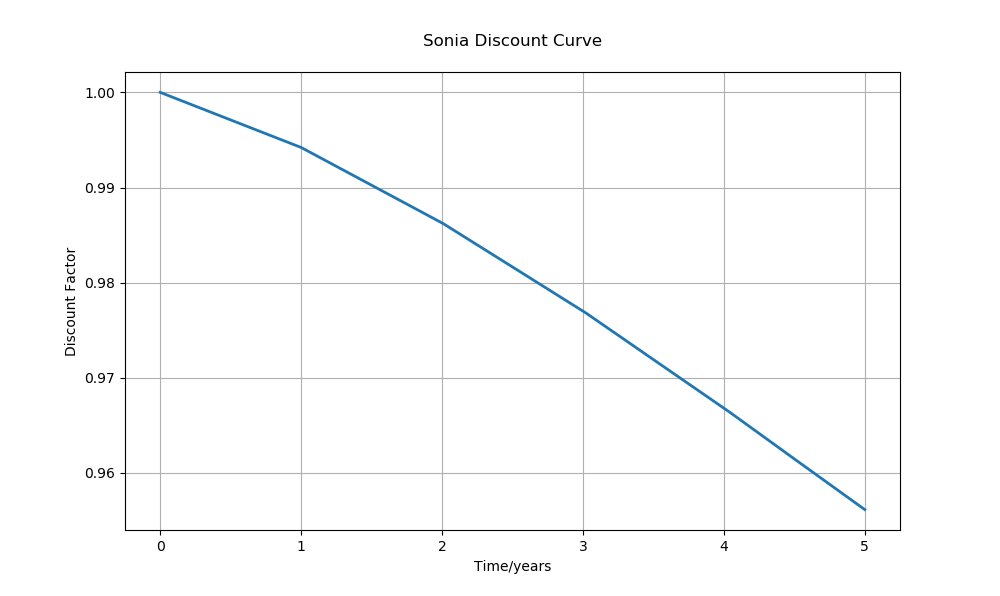
\includegraphics[width=15cm]{Sonia_Discount_Curve.png}
		\caption{SONIA Discount Curve} 
		\label{Sonia_Discount_Curve}
	\end{center}
\end{figure}

\chapter{Implied Probability of Default}
In order to estimate the default probabilities for each of the probabilities and hence the term structure of hazard rates, we bootstrap survival probabilities from the Credit Spreads data as follows:

\begin{align*}
\mathbf{S}_n := \frac{\sum_{i=1}^{n-1}DF_{\tau_i} \cdot \Big[ (1-R)\mathbf{S}_{i-1} - \mathbf{S}_{i}(1 - R + \psi_n(\tau_i - \tau_{i-1}))  \Big]  }{ DF_{\tau_n} (1 - R + \psi_n(\tau_n - \tau_{n-1})) } + \frac{\mathbf{S}_{n-1}(1-R)}{1 - R + \psi_n(\tau_n - \tau_{n-1})}
\end{align*}
where:
\begin{itemize}
	\item $N$ is the number of credit spreads of differing tenor that I have available to me from the market.
	\item $n \in {1,...,N}$ 
	\item $R$ is the Recovery rate which is defined in the market to be at 40\% for these credit spreads.
	\item $\tau_n$ is defined as the $n^{th}$ tenor where $\tau_{n-1} \le \tau_{n} \forall n \in {2,...,N}$.
	\item $DF_{\tau_n}$ is a factor that discounts in pounds sterling from $\tau_n$ to present.
	\item $\psi_n$ is defined as the $n^{th}$ credit spread.
	\item $\mathbf{S}_n$ as the $n^{th}$ survival probability implied by $\psi_n$.
	\item $\mathbf{S}_0 := 1$ 
	\item $\mathbf{S}_1 := \frac{\mathbf{S}_{0}(1-R)}{1 - R + \psi_1(\tau_1 - \tau_{0})}$ 
\end{itemize}

With equivalent hazard rates, $\lambda_n$, as follows:
\begin{align*}
\lambda_n = -\frac{log(\mathbf{S}_n/\mathbf{S}_{n-1})}{\tau_{n} - \tau_{n-1}}
\end{align*}
for $n \in {1,...,N}$ where $\lambda_n$ is defined as the hazard rate in the time interval $[\tau_{n-1},\tau_n)$.\\

From the market credit spreads, I calculate the following implied term structure of hazard rates:

\begin{figure}[H]
	\begin{center}
		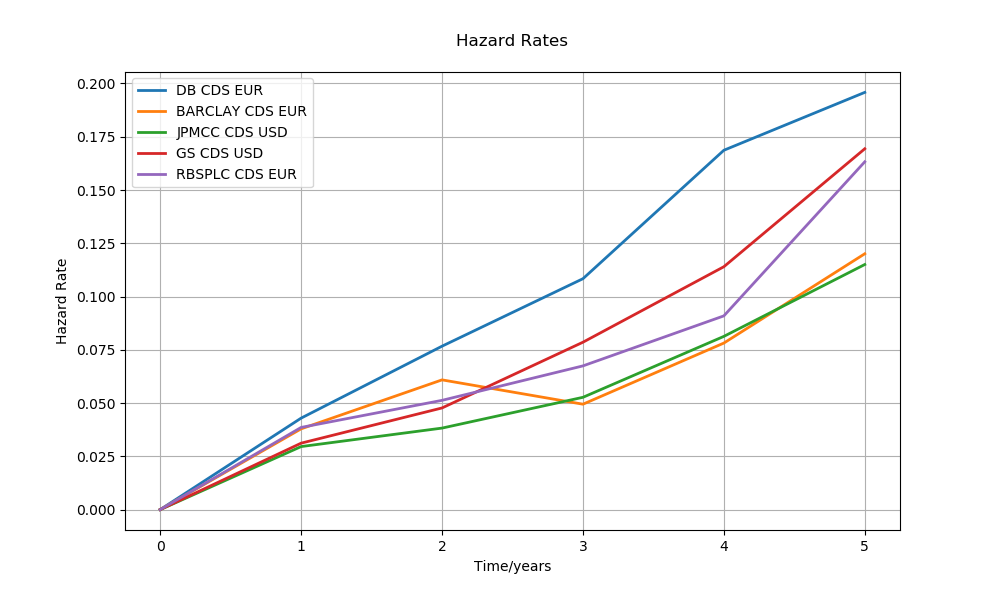
\includegraphics[width=15cm]{Hazard_Rates.png}
		\caption{Term structure of hazard rates for each reference name} 
		\label{Hazard_Rates}
	\end{center}
\end{figure}


\chapter{Correlations \& Copula Parametrisation}

I now estimate the correlations between the default probability of each of the reference names. As the default probability correlation between 2 reference names is not dependent on the tenor, but instead on the relationship between the 2 reference names (i.e. positions with one-another), we use the most liquid tenor at 5 years of historical credit spreads for deriving the probability of default correlations as we can compare this data for each reference name side-by-side. It is however worth noting that Credit spreads depend on other external market influences than just the default probability of a company as they are a traded instrument; therefore, credit spreads are not necessarily a perfect indicator for the default probability correlation structure between counterparties. But due to data constraints and the fact that default probabilities themselves are not directly 'tradable' (not observable); I will use credit spreads as other methods of deriving correlations are outside of the scope of this project.\\

\section{Default Correlations (Canonical Maximum Likelihood}

\begin{figure}[H]
	\begin{center}
		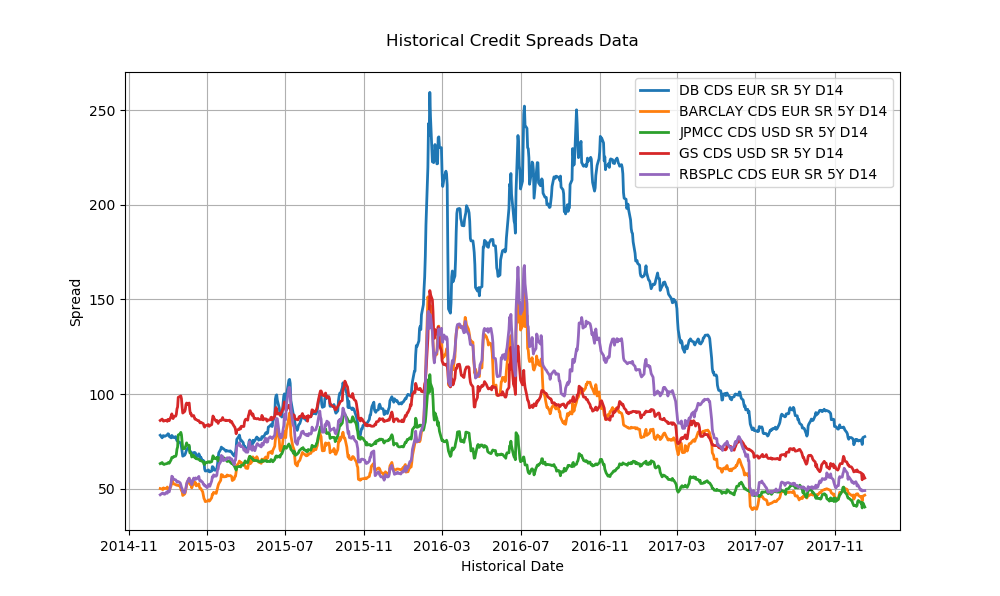
\includegraphics[width=15cm]{Historical_Credit_Spreads_Data.png}
		\caption{Historical Credit Spreads Data} 
		\label{Historical_Credit_Spreads_Data}
	\end{center}
\end{figure}

To calculate the correlation matrix, I begin by calculating log returns from the historical credit spreads for each reference name (as seen in figure \ref{Historical_Credit_Spreads_Data} above). I calculate the \textbf{weekly} returns to begin with as I believe that the weekly returns will have significantly less noise than daily returns. Considering that there needs to be sufficient data to calculate meaningful correlations that don't change wildly based on sample size, I choose arbitrarily to use at least 100 data points to calculate correlations from; this results in historical spreads from at least 2 years back. 

\begin{align*}
rln_{ji} = Log(\psi_{ji} / \psi_{ji - l}) \text{ UPDATE TO AVERAGE FROM CODE}
\end{align*}
where:
\begin{itemize}
	\item $i$ indexes each day in the historical data. Meaning that $ji$ gives results in the calculation of one return every $j$ business days. I begin by setting $j = 1$.
	\item $l$ is the lag in numbers of days. I use a lag of 5 to result in weekly returns.
	\item $rln$ is the log return.
\end{itemize}

\subsection{Pearson Correlation}

For the Gaussian copula, I calculate the \textbf{Linear, (Pearson)} correlation, $\mathbf{C}^{lin}$, between log returns and use this to parametrise the copula. Using linear correlation as a measure of co-dependance is only acceptable when the underlying variables are Gaussian. Therefore we will use the linear correlation to parametrise the Gaussian copula. Furthermore, for linear correlations the following hold:

\begin{itemize}
	\item A correlation of 0 is equivalent to independence for Gaussian distributions.
	\item Given elliptical marginal distributions and their correlation, it is possible to construct a joint distribution.
\end{itemize}

I calculate the log of the credit spreads historical \emph{weekly} returns for each reference name as below:

\begin{figure}[H]
	\begin{center}
		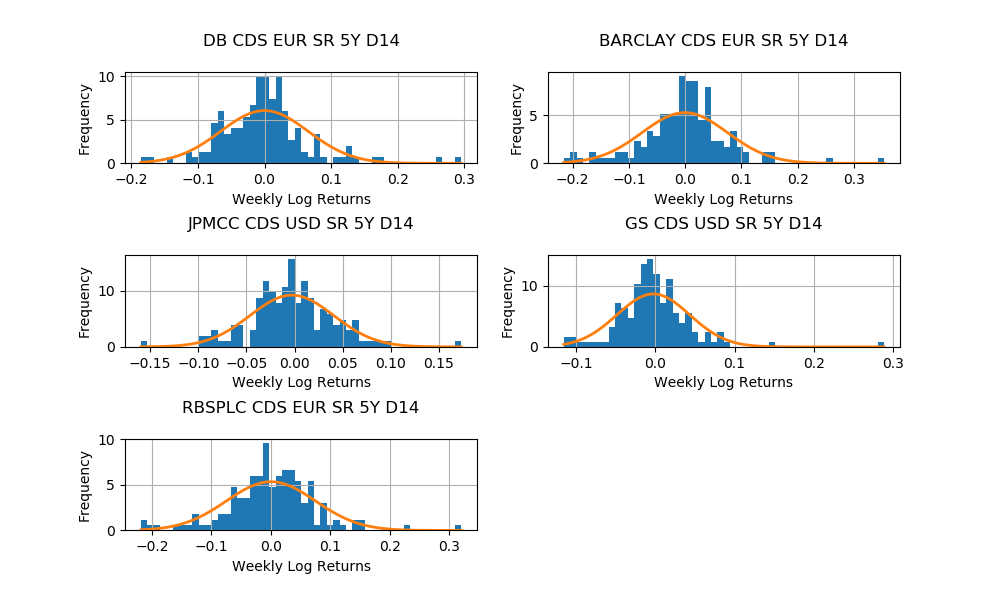
\includegraphics[width=15cm]{Weekly_log_returns.png}
		\caption{Weekly Log Returns} 
		\label{Weekly_log_returns}
	\end{center}
\end{figure}

In doing so, I am able to calculate a Pearson correlation matrix: 

\begin{center}
	\begin{tabular}{|l|l|l|l|l|c|c|c|c|c|}
		\hline
		& \textbf{0} & \textbf{1} & \textbf{2} & \textbf{3} & \textbf{4}\\\hhline{|=|=|=|=|=|=|}
		\textbf{0} & 1.0 & 0.816648231202 & 0.494174976017 & 0.604054027376 & 0.799331842251\\
		\textbf{1} & 0.816648231202 & 1.0 & 0.516350004433 & 0.589791041796 & 0.938783819003\\
		\textbf{2} & 0.494174976017 & 0.516350004433 & 1.0 & 0.883763607982 & 0.509473862112\\
		\textbf{3} & 0.604054027376 & 0.589791041796 & 0.883763607982 & 1.0 & 0.582036956658\\
		\textbf{4} & 0.799331842251 & 0.938783819003 & 0.509473862112 & 0.582036956658 & 1.0\\
		\hline
	\end{tabular}
\end{center}

\subsection{Rank Correlation}

On the other hand, for the Student's t copula, the underlying variables are not Gaussian and so using the linear correlation would be unsuitable here. Instead I use the \textbf{Rank} correlation because this gives scale invariant estimates of the correlation which are more suitable for non-Gaussian random variables. Intuitively, the rank correlation measures the dependency between a big movement in one reference name's credit spread in comparison to a movement of equivalent ranking in another reference name's credit spread. I calculate \textbf{Spearman's Rho}, which is a rank correlation, by \emph{ranking} the observations in order and then scaling them to $[0,1]$ to output scale invariant estimates of the correlation. An alternative Rank correlation that can also be used is \textbf{Kendall's Tau}. As stated above, this is important for the student's t copula because the student's t distribution does not satisfy the constraints of the linear correlation above. \\

To calculate the Rank correlation, I first compute the absolute differences from the historical credit spreads for each reference name which are near-Gaussian distributed. I then calculate the Empirical CDF of these differences and use it to transform the data (\textit{absolute differences}). This is known as \emph{Canonical Maximum Likelihood Estimation}. The downside of this non-parametric method is that the Uniform samples obtained from the transformed data may not be sufficiently uniform which leads to gaps in the resulting copula (joint distribution of defaults). The absolute differences are given by:

\begin{align*}
\text{diff}_{ji} = |\psi_{ji} - \psi_{ji - l}| UPDATE TO AVERAGE
\end{align*}
where diff is the absolute differences for historical day $(ji)$.\\

I calculate the weekly Absolute differences taking the average of each week and subtracting week-on-week; the resulting differences have the following distributions:

\begin{figure}[H]
	\begin{center}
		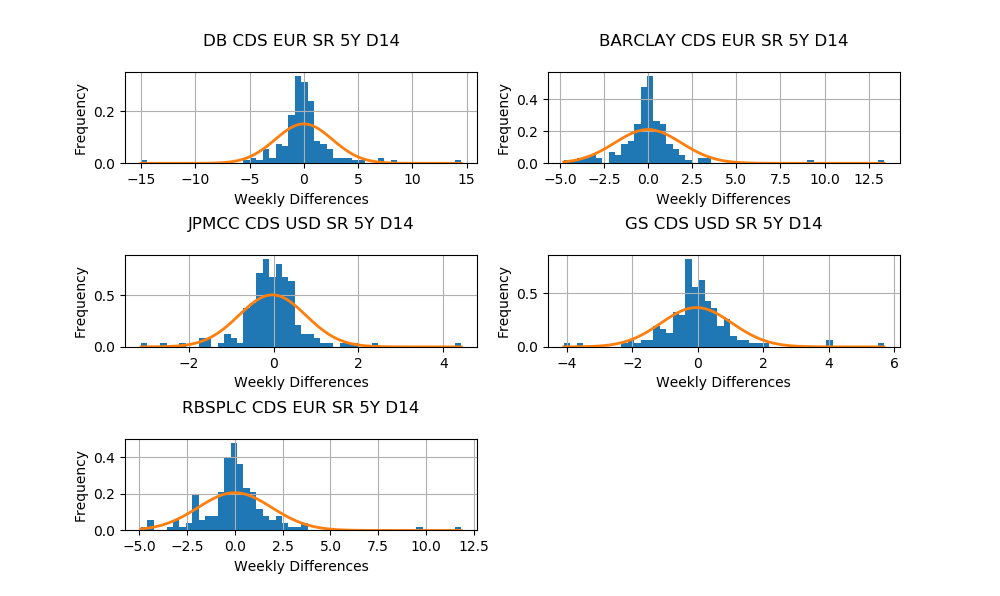
\includegraphics[width=15cm]{Weekly_absolute_diffs.png}
		\caption{Weekly Absolute Differences} 
		\label{Weekly_absolute_diffs}
	\end{center}
\end{figure}

The Empirical Cumulative Distribution function (ECDF) is given by:

\begin{align*}
\hat{F}_n(t) := \frac{1}{n}\sum_{i=1}^{n}1_{x_i \leq t}
\end{align*}
where $n$ is the sample size and $i$ indexes the sample.\\

We see from the below histograms, that the transformed data is approximately uniform as expected:

\begin{figure}[H]
	\begin{center}
		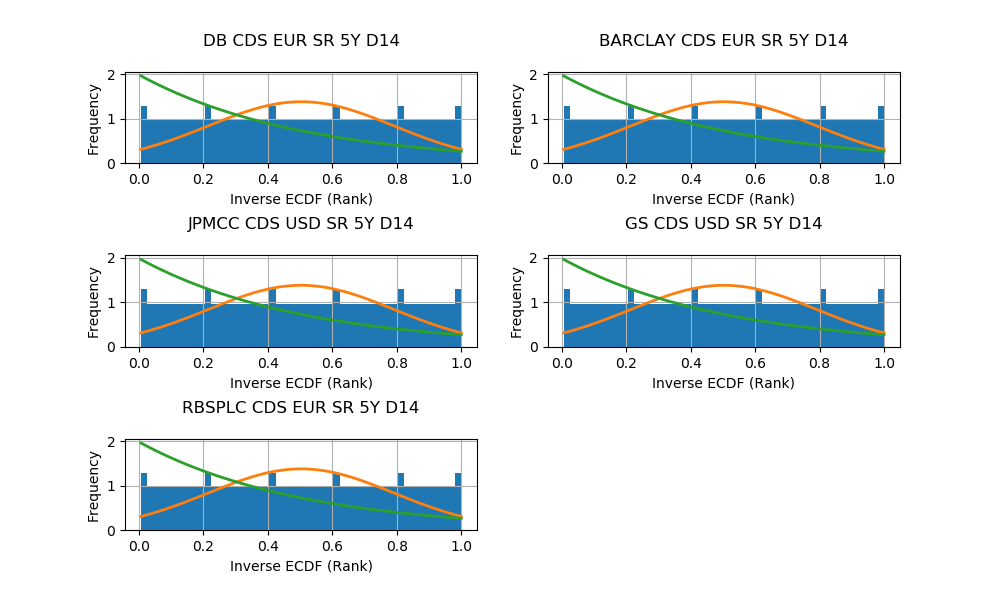
\includegraphics[width=15cm]{Inverse_ECDF_Rank.png}
		\caption{Distribution of Differences by their ECDF} 
		\label{Inverse_ECDF_Rank}
	\end{center}
\end{figure}

The Rank correlation, $\mathbf{C}^{rank}$, is then calculated from the transformed differences:

\begin{center}
	\begin{tabular}{|l|l|l|l|l|c|c|c|c|c|}
		\hline
		& \textbf{0} & \textbf{1} & \textbf{2} & \textbf{3} & \textbf{4}\\\hhline{|=|=|=|=|=|=|}
		\textbf{0} & 1.0 & 0.749581956979 & 0.407502315046 & 0.46285660097 & 0.749496609821\\
		\textbf{1} & 0.749581956979 & 1.0 & 0.461372496454 & 0.439417742726 & 0.914870951937\\
		\textbf{2} & 0.407502315046 & 0.461372496454 & 1.0 & 0.870027140204 & 0.479936211549\\
		\textbf{3} & 0.46285660097 & 0.439417742726 & 0.870027140204 & 1.0 & 0.482050228383\\
		\textbf{4} & 0.749496609821 & 0.914870951937 & 0.479936211549 & 0.482050228383 & 1.0\\
		\hline
	\end{tabular}
\end{center}

I display the difference between the 2 correlation matrices below which shows that in general, the correlation matrices roughly agree as the differences are not in general large. The  largest difference appears between Deutsche Bank and RBS with a difference of -0.0498 which can be explained by the differences in the scales of the credit spreads of the 2 reference names. The Pearson correlation does not take scaling into account:

\begin{center}
	\begin{tabular}{|l|l|l|l|l|c|c|c|c|c|}
		\hline
		& \textbf{0} & \textbf{1} & \textbf{2} & \textbf{3} & \textbf{4}\\\hhline{|=|=|=|=|=|=|}
		\textbf{0} & 0.0 & -0.0670662742229 & -0.0866726609714 & -0.141197426406 & -0.0498352324296\\
		\textbf{1} & -0.0670662742229 & 0.0 & -0.0549775079796 & -0.15037329907 & -0.0239128670659\\
		\textbf{2} & -0.0866726609714 & -0.0549775079796 & 0.0 & -0.0137364677779 & -0.0295376505625\\
		\textbf{3} & -0.141197426406 & -0.15037329907 & -0.0137364677779 & 0.0 & -0.0999867282749\\
		\textbf{4} & -0.0498352324296 & -0.0239128670659 & -0.0295376505625 & -0.0999867282749 & 0.0\\
		\hline
	\end{tabular}
\end{center}

\section{Extreme Value Theory}

It is often the case that financial data is not well represented in the tails of a Gaussian distributions. To solve this shortcoming, one can employ Extreme Value Theory (EVT). EVT is a statistical tool to deal with extreme deviations from a distribution's median. In general, EVT is used to characterise the distribution of a sample maximum of a distribution values above a certain threshold (tail(s)).\\ 
%Paper: Modeling TAil Behaviour with Extreme Value Theory by Damon Levine from Risk Management Journal.
Here we use a Generalised Pareto Distribution (GPD) to model the tail(s). The Picklands-Balkema-de Haan Theorem, stated below, supports this choice.\\ 
When employing Extreme value theory to model the tails, I apply a semi-parametric fit to the centre of the data sample using Kernel Smoothing which is a parametric alternative to a histogram.\\

\subsection{Kernel Smoothing}

% Add https://mglerner.github.io/posts/histograms-and-kernel-density-estimation-kde-2.html?p=28 to references.
Kernel smoothing is a parametric method of density estimation. Like a histogram (non-parametric density estimation), kernel smoothing looks to create a distribution for the data based on which section (bin) of the data each sampling unit fits within. The difference between the two is that a histogram:
\begin{itemize}
	\item predefines discrete bins for this data which heavily influences the observed distribution of the data.
	\item is \emph{very} dependent on the choice of boundaries for each bin.
\end{itemize}
%http://www.mvstat.net/tduong/research/seminars/seminar-2001-05/
On the other hand, kernel smoothing:
\begin{itemize}
	\item does not depend on the boundaries of bins as all the theoretical bins are recentred for each sampling unit.
	\item is, as the name suggests, a smooth density estimation.
	\item can take an optimal bandwidth using estimates such as by minimising the optimality criterion: \textit{Asymptotic Mean Integrated Squared Error} which is defined below.
\end{itemize}

\begin{defn}
	\textbf{Kernel density estimation}:\\
	$K(x)$ is defined as the chosen kernel which is a non-negative function that integrates to one. $h$ is defined as the bandwidth of the KDE. First I define $(x_1,...,x_n)$ to be sampled from some distribution with unknown distribution $f(x)$, $x_i$ are univariate independent and identically distributed, the kernel density estimator is then defined as follows: 
	\begin{align*}
	\hat{f}_h(x) := \frac{1}{nk} \sum_{i=1}^{n}K\Big(\frac{x - x_i}{h}\Big)
	\end{align*}
\end{defn}

\begin{defn}
	The \textbf{Mean Integrated Squared Error} is defined as follows to estimate the optimal bandwidth, $\hat{h}$:
	\begin{align*}
	MISE(h) = \mathbf{E}\Big[ \int (\hat{f}_h(x) - f(x))^2 dx \Big]
	\end{align*}
\end{defn}	
\begin{defn}
	The \textbf{Asymptotic Mean Integrated Squared Error} is then defined as follows:
	\begin{align*}
	AMISE(h) = \frac{\int (K(x))^2 dx}{nh^2} + \frac{1}{4}\mathbf{E}_K[X^2]h^4\int (f^{''}(x))^2 dx
	\end{align*}
\end{defn}

I will use $\hat{f}_h(x)$ to estimate the centre of the density of CDS returns.

\subsection{Generalised Pareto Distribution}

\begin{thm}
	\textbf{Picklands-Balkema-de Haan}:\\
	For a very large family of distributions, for a sufficiently large threshold value, $u$, and data points $p_i \ \forall i \in \{1,...,n\}$ where $n$ is the number of points; the distribution of excesses, $(p_i - u)$, is well approximated by a \emph{Generalised Pareto Distribution}.\\
	This family of distributions includes Gaussian, lognormal, beta, exponential, F, gamma, Student t uniform...
\end{thm}

To apply the theorem above to the left tail or both tails, we consider the absolute excesses, $|p_i - u|$, instead.

\begin{defn}
	\textbf{GPD CDF}:\\
	\begin{equation}
	G_{k,\mu,s} (x) := \left\{
	\begin{array}{@{}ll@{}}
	1 - (1 - k(x-\mu)/s)^{1/k}, & \text{if}\ k \ne 0 \\
	1 - exp(-(x-\mu)/s), & \text{otherwise}
	\end{array}
	\right.
	\end{equation} 
	where 
	\begin{itemize}
		\item $k$ is the shape of the distribution.
		\item $\mu$ is the location of the distribution (i.e. for modelling excesses will most likely start near 0+).
		\item $s$ is the scale of the distribution (a variance parameter).
	\end{itemize}
\end{defn}

\subsection{Semi-parametric fitting}

With GPD defined above, one can define a CDF modelling the entire data set as follows: 
\begin{equation}
F(x) := \left\{
\begin{array}{@{}ll@{}}
F_n(u)\Big[1-G(u-x)\Big], & \text{if}\ x < u \\
\Big[1 - F_n(u)\Big]G(x-u) + F_n(u), & \text{if}\ x \geq u \\
F_n(x), & \text{otherwise}
\end{array}
\right.
\end{equation}
where $F_n(x)$ is a function that estimates the centre of the distribution and integrates to 1. This implies the PDF:
\begin{equation}
f(x) := \left\{
\begin{array}{@{}ll@{}}
F_n(u)g(u-x), & \text{if}\ x < u \\
\Big[1 - F_n(u)\Big]g(x-u), & \text{if}\ x \geq u \\
f_n(x), & \text{otherwise}
\end{array}
\right.
\end{equation}
where $g(x) := \frac{d}{dx}(G(x))$.

\begin{exmp}
	Example of test data and how the parametric fit compared to actual gaussian mix
\end{exmp}

\subsubsection{Choosing the Threshold, u}
I choose the 95\% percentile of the sample data as a value for $u$ because I obtain excesses from both tails which gives me 10\% of the data to fit the GPD. To parametrise the GPD, the \emph{method of moments} is used.

%INclude Plots of Fits here.

\subsection{Semi-parametric Revised Rank Correlation}

I fit the Historical Credit Spread Data using my implementation of the Semi-parametric fit described above which results in the data having been transformed by it's own (semi-parametric) CDF. I then recalculate the correlation matrix from these values which is given below:

\begin{center}
	\begin{tabular}{|l|l|l|l|l|c|c|c|c|c|}
		\hline
		& \textbf{0} & \textbf{1} & \textbf{2} & \textbf{3} & \textbf{4}\\\hhline{|=|=|=|=|=|=|}
		\textbf{0} & 1.0 & 0.873078750958 & 0.158978473828 & 0.620707344076 & 0.882818382128\\
		\textbf{1} & 0.873078750958 & 1.0 & 0.427120471404 & 0.823583184822 & 0.975301584703\\
		\textbf{2} & 0.158978473828 & 0.427120471404 & 1.0 & 0.763272964379 & 0.337685521639\\
		\textbf{3} & 0.620707344076 & 0.823583184822 & 0.763272964379 & 1.0 & 0.757861144396\\
		\textbf{4} & 0.882818382128 & 0.975301584703 & 0.337685521639 & 0.757861144396 & 1.0\\
		\hline
	\end{tabular}
\end{center}

The revised correlation matrix is calculated from 5 times as many data points as we don't look at weekly returns for the revised correlation. This gives us a consistently more extreme pairwise correlations.\\

To perform a direct comparison, I take the difference between the revised and the original rank correlation:

\begin{center}
	\begin{tabular}{|l|l|l|l|l|c|c|c|c|c|}
		\hline
		& \textbf{0} & \textbf{1} & \textbf{2} & \textbf{3} & \textbf{4}\\\hhline{|=|=|=|=|=|=|}
		\textbf{0} & 0.0 & 0.123496793979 & -0.248523841217 & 0.157850743105 & 0.133321772306\\
		\textbf{1} & 0.123496793979 & 0.0 & -0.0342520250493 & 0.384165442096 & 0.0604306327659\\
		\textbf{2} & -0.248523841217 & -0.0342520250493 & 0.0 & -0.106754175825 & -0.142250689909\\
		\textbf{3} & 0.157850743105 & 0.384165442096 & -0.106754175825 & 0.0 & 0.275810916013\\
		\textbf{4} & 0.133321772306 & 0.0604306327659 & -0.142250689909 & 0.275810916013 & 0.0\\
		\hline
	\end{tabular}
\end{center}

I now reconsider the difference matrix between the revised rank correlation and the pearson correlation below:

\begin{center}
	\begin{tabular}{|l|l|l|l|l|c|c|c|c|c|}
		\hline
		& \textbf{0} & \textbf{1} & \textbf{2} & \textbf{3} & \textbf{4}\\\hhline{|=|=|=|=|=|=|}
		\textbf{0} & 0.0 & 0.0564305197565 & -0.335196502189 & 0.0166533166992 & 0.0834865398768\\
		\textbf{1} & 0.0564305197565 & 0.0 & -0.0892295330289 & 0.233792143026 & 0.0365177657\\
		\textbf{2} & -0.335196502189 & -0.0892295330289 & 0.0 & -0.120490643603 & -0.171788340472\\
		\textbf{3} & 0.0166533166992 & 0.233792143026 & -0.120490643603 & 0.0 & 0.175824187738\\
		\textbf{4} & 0.0834865398768 & 0.0365177657 & -0.171788340472 & 0.175824187738 & 0.0\\
		\hline
	\end{tabular}
\end{center}

Note the sizeable change in the Deutsche Bank - JPMorgan correlation of -0.335196502189 from -0.0866726609714 before.

\section{Random number generation}

To sample from the parametrised copulas, one needs to be able to sample random variables from U[0,1]. Computationally, the following random number generation techniques are commonly used:
\begin{itemize}
	\item Pseudo-random numbers.
	\item Low discrepancy numbers.
\end{itemize}

Pseudo random numbers use number theory to generate \emph{a sequence of random numbers} on an $n$-dimensional plane where the only restriction on the elements of the sequence is that they are constrained to the plane. Each sequence is uniquely defined by a unique seed (number) that is arbitrarily chosen outside of the scope of the generator.\\

%Low discrepancy numbers again use number theory to generate \emph{a sequence of linked random numbers} on an $n$-dimensional plane with the same constraints as Psuedo-random numbers. 
Low discrepancy numbers are a subset of pseudo-random numbers. They have the additional feature that each new element in the sequence is generated to be maximise the modulus of the difference between the new element and all other elements in the sequence. This ensures that Low discrepancy numbers spread over the plane much quicker than Pseudo-random numbers which can cluster. It is a useful feature for Monte Carlo simulation as one can achieve convergence of the estimate in far fewer simulations.\\

%Plot the comparison between Pseudo random scatters at iterations, 5, 50, 200 and Low discrepancy numbers scatters.

In this project, we will use \textbf{Sobol numbers} which are a type of low discrepancy numbers.

\section{Sobol numbers}

I briefly outline the generation of Sobol numbers. The algorithm has not been tweaked from the literature as it is very sensitive and number theory is outside of the scope of this project.\\

\begin{enumerate}
	\item Start with integers on the interval $[1,2^b-1]$ where $b=32$ representing the 32 bits of the x86 language that I use to generate the sequence. 
	\item Define $x_{nk}$ to be the $n^{th}$ draw of the $k^{th}$ dimension of the sequence. Then $y_{nk} := \frac{x_{nk}}{2^b}$ where $y_{nk} \in (0,1]$
	\item I next define the \emph{direction integers} which are the underlying basis of the number generation. Define $v_{kl}$ to be the $l^{\text{th}}$ direction integer for dimension $k$. These direction integers are constrained to the following rules: 
	\begin{itemize}
		\item Only the $l$ left-most bits of the bitfield for $v_{kl}$ can be non-zero.
		\item The $l^{\text{th}}$ bit must be set.
	\end{itemize}
	\item Define the \textit{primitive polynomial} $p_k(z) := \sum_{j=0}^{g_k} a_{kj}z^{g_k-j}$ where $g_k$ is the dimension of the polynomial, $p_k(z)$.
	\item For a given dimension $k$ with primitive polynomial $p_k(z)$, we have the following: 
	\begin{itemize}
		\item For $l \in \{1,...,g_k\}$, $v_{kl}$ are \textbf{initialised} freely. I discuss this initialisation process below.
		\item For $l\ge g_k$: $$v_{kl} = \frac{v_{k(l-g_k)}}{2^{g_k}} \oplus_2 {\sum_{j=1}^{g_k}}^{\oplus_2} a_{kj}v_{k(l-j)}$$
	\end{itemize}
	\item Then as in other number generators, for each draw, $n$, one requires a generating integer $\gamma(n)$. It is common and simple to choose $\gamma(n) = n$; however I discuss below that it is far more efficient to choose $\gamma(n) = G(n)$ where $G(n)$ is the \textbf{Gray Code}. I explain the Gray Code below. Thus my implementation of the generator uses the Gray Code.
	\item Then finally: 
	\begin{equation}
	\label{soboleqn}
	x_{nk} := {\sum_{j=1}^{d}}^{\oplus_2} v_{kj}\mathcal{1}_{\{j^{th} bit of \gamma(n) is set\}}
	\end{equation}
\end{enumerate}

\subsection{Gray code integer encoding}

Gray Code is an encoding of integers for efficiency in computational iterators / algorithms. The idea is that for each integer $n$, $\exists$ as bitwise representation of $n$ such that the bitwise representation of $(n+1)$ differs by only \textbf{one} bit. I define this representation to be $G(n)$. Furthermore, the one bit that differs is the right-most zero bit of $n$. \\

The Gray Code is \emph{not} unique. In my implementation, I use a commonly version of the encoding: $G(n) := n \oplus_2 [n/2]$. Then, because $G(n)$ differs from $G(n+1)$ by one bit, only \emph{one} of the operations in equation \ref{soboleqn} is necessary. Therefore: $$ x_{nk} = x_{(n-1)k} \oplus_2 v_{jk}$$

\subsection{Initialisation}

I remind the reader of the initialisation of the direction integers which is a problem with many solutions. The behaviour and properties of the generated sequence is heavily dependent on the choice of initialisation of the direction integers. In order to review the quality of an initialisation, I introduce the following number theory definition.

\begin{defn}
	\textbf{Property A (dispersion)} states that a low discrepancy is said to have property A if for any binary segment (not an arbitrary subset) of the $d$-dimensional sequence of length $2^d$, there is exactly one draw in each of the $2^d$ hypercubes that result from subdividing the unit hypercube along each of its unit length extensions into half.
\end{defn}

The simplest initialisation is \textbf{Unit initialisation} which is easy to implement but leads to poorly generated sequences. Unit initialisations sets: $$v_{kl} = 2^{b-l}$$
Instead, one can use \textbf{Pseudo-random initialisation} which uses a separate pseudo-random number generator to generate $u_{kl}^* \sim U[0,1]$. One then defines $w_{kl} = int(u_{kl}^* \cdot 2^{l-1})$ where $int(x)$ is a function that rounds $x$ to the nearest integer and $w_{kl}$ is only used when it satisfies $w_{kl} \% 2 = 1$. Then: $$v_{kl} = w_{kl} \cdot 2^{b-l}$$
I use the pseudo-random initialisation in my implementation as the behaviour of the generator is much better than unit initialisation.

\section{Copula Parametrisation \& Calculation}
%See slide 48 of CDO And Copula Models presentation.\\

To use the copulas in the Monte Carlo simulation, one only needs to simulate Uniform random variables from the underlying copula within the scope of this project. With this in mind, the following algorithms are implemented to parametrise the underlying copula using the correlation of reference name defaults and then simulate Uniform random variables.\\

To start with, I apply the following to simulate from the underlying Gaussian copula:
\begin{enumerate}
	\item Apply \emph{matrix decomposition} to the Correlation matrix, $\Sigma$: $\Sigma = A A^{T}$
	\item Simulate $n$, where $n$ is the number of reference names, random draws from a uniform distribution, $U$ using a low discrepancy number generator.
	\item Convert the Uniform random variables to standard normal random variables, $Z$, by applying the inverse standard normal CDF.
	\item Convert the standard normal variables to correlated normal variables: $X = AZ$
	\item Apply the \emph{inverse marginal CDF} (Gaussian CDF) to each correlated normal variable to obtain the simulated default time for each reference name.
\end{enumerate}

To simulate from the underlying Students T copula, I apply the steps above excluding the final marginal transformation; I then apply the following additional steps to simulate from the Students T copula:
\begin{enumerate}
	\item Draw a vector of squared uniform random variables $\bar{u}$ of length equal to the degrees of freedom, $df$, of the underlying Students T copula.
	\item Next create a new scaled vector of correlated random variables by transforming each correlated standard normal random variable from above by: $\Psi := X / \sqrt{\frac{\sum_{i=0}^{(df-1)}\bar{u}_i}{\epsilon}}$
	\item Apply the \emph{inverse marginal CDF} (Students T CDF) to each scaled correlated normal variable ($\Psi$) to obtain the simulated default time for each reference name.
\end{enumerate}


\chapter{Simulation \& Observations}

\section{Estimation of Fair Spread by simulation}

\subsection{Reference name co-dependencies}

Having computed default probabilities and discount factors, I first parametrise the copulas. I observe the following co-dependencies between the reference names from observing the copulas:

\begin{figure}[H]
	\begin{center}
		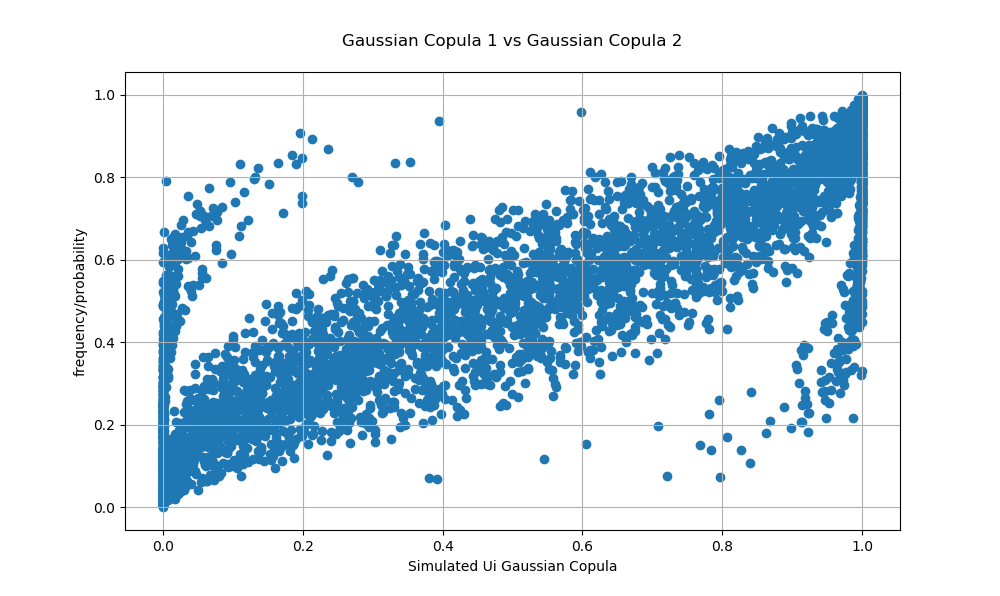
\includegraphics[width=15cm]{Gaussian_Copula_1_vs_Gaussian_Copula_2.png}
		\caption{Joint Distribution of 1st and 2nd reference names in the Gaussian Copula} 
		\label{Gaussian_Copula_1_vs_Gaussian_Copula_2}
	\end{center}
\end{figure}

I expect that the relationship between $U_1$ (The transformed Uniform R.V.s from the Deutsche Bank credit spread returns) and $U_2$ (Barclays) should resemble the pattern of an elliptical copula density to confirm that elliptical Copulas satisfy the dependence structure of the transformed historical data. Figure \ref{copulademo_08} is taken from  \href{http://www.mbfys.ru.nl/~robvdw/CNP04/LAB_ASSIGMENTS/LAB05_CN05/MATLAB2007b/stats/html/copulademo.html}{mbfys} to show a classic scatter of the marginals of an elliptical copula so that one can compare the two plots.

\begin{figure}[H]
	\begin{center}
		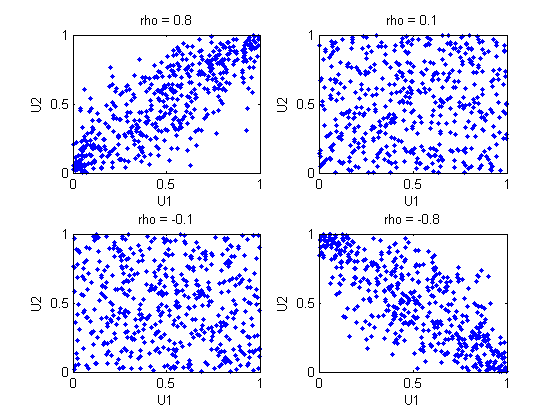
\includegraphics[width=15cm]{copulademo_08.png}
		\caption{Joint Distribution of 1st and 2nd marginals from Elliptical Copula. \newline Taken from \href{http://www.mbfys.ru.nl/~robvdw/CNP04/LAB_ASSIGMENTS/LAB05_CN05/MATLAB2007b/stats/html/copulademo.html}{here}.} 
		\label{copulademo_08}
	\end{center}
\end{figure}

I note that Figure \ref{Gaussian_Copula_1_vs_Gaussian_Copula_2} differs from Figure \ref{copulademo_08} in its tails. So Extreme Value Theory (EVT) can be applied here to tackle this data structure issue.

\begin{figure}[H]
	\begin{center}
		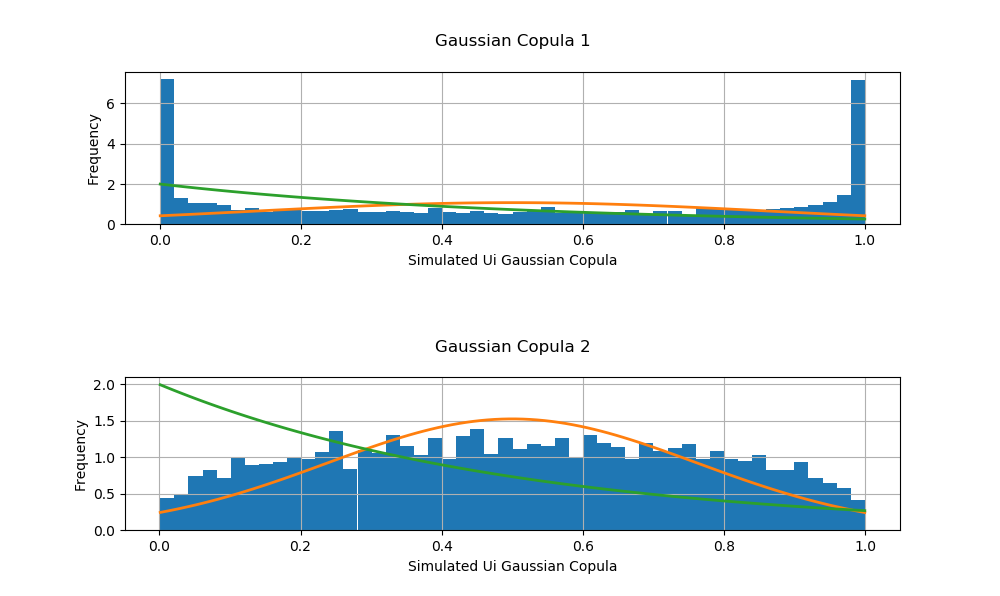
\includegraphics[width=15cm]{Gaussian_Copula_1.png}
		\caption{Marginal Distributions of 1st and 2nd reference name in the Gaussian Copula} 
		\label{Gaussian_Copula_1}
	\end{center}
\end{figure}

\begin{figure}[H]
	\begin{center}
		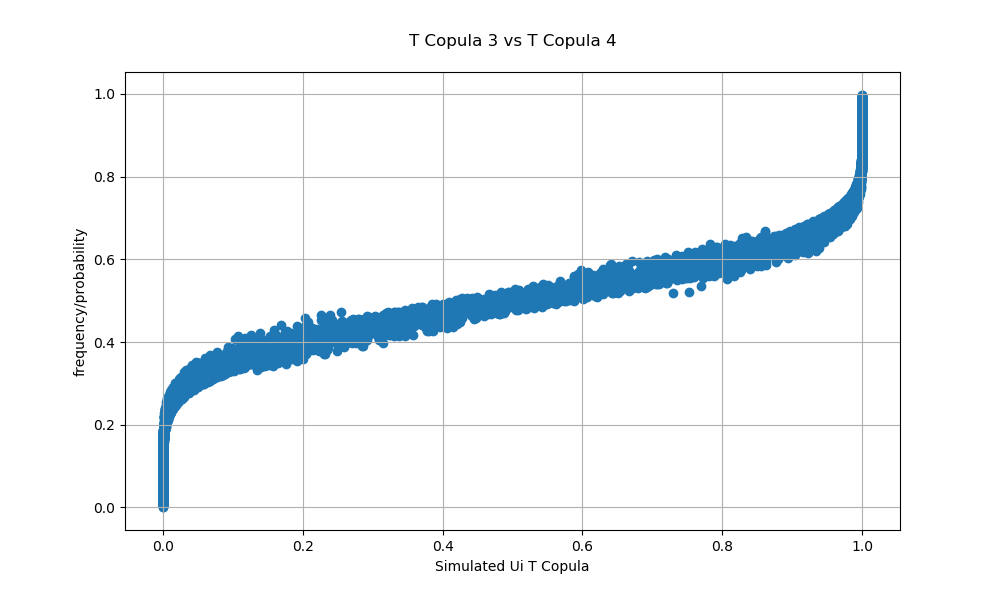
\includegraphics[width=15cm]{T_Copula_3_vs_T_Copula_4.png}
		\caption{Joint Distribution of 3rd and 4th reference names in the Student's T Copula} 
		\label{T_Copula_3_vs_T_Copula_4}
	\end{center}
\end{figure}

\begin{figure}[H]
	\begin{center}
		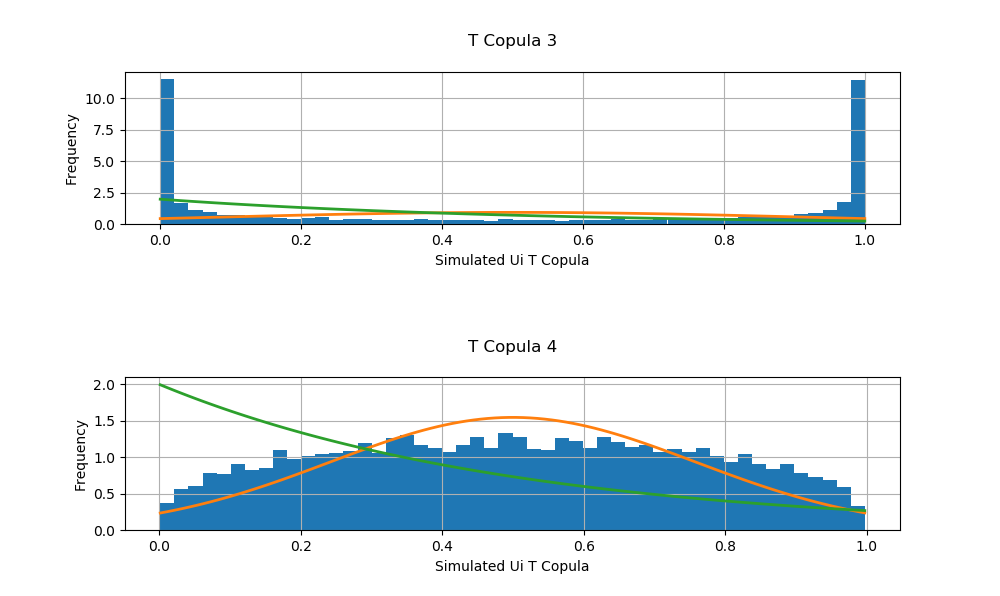
\includegraphics[width=15cm]{T_Copula_3.png}
		\caption{Marginal Distributions of 3rd and 4th reference name in the Student's T Copula} 
		\label{T_Copula_3}
	\end{center}
\end{figure}


\subsection{Monte-Carlo Observations}

I now run the simulation where the running averages and running variances are displayed below. This illustrates the benefit of using Low discrepancy numbers because one observes that the conversion of the Monte Carlo estimate occurs in far fewer iterations when the simulation contains a relatively small number of dimensions. \textit{Note that the Monte Carlo simulations were stopped before the maximum number of iterations of 5000 if they converged, this is the reason for the running averages falling suddenly to 0.}

\begin{figure}[H]
	\begin{center}
		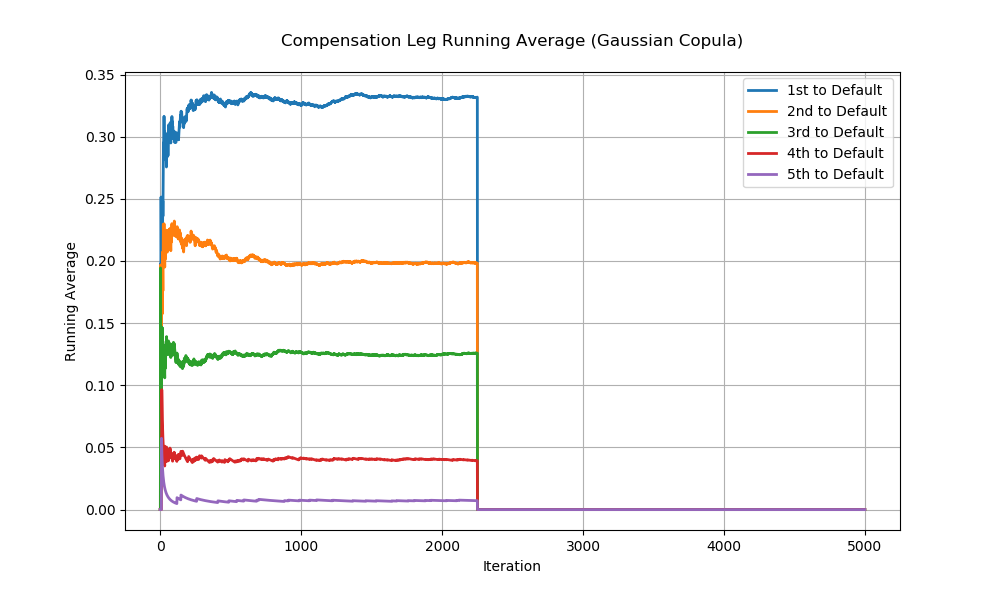
\includegraphics[width=15cm]{Compensation_Leg_Running_Average_(Gaussian_Copula).png}
		\caption{Running Average of Compensation Leg for the Gaussian Copula} 
		\label{Compensation_Leg_Running_Average_(Gaussian_Copula)}
	\end{center}
\end{figure}

\begin{figure}[H]
	\begin{center}
		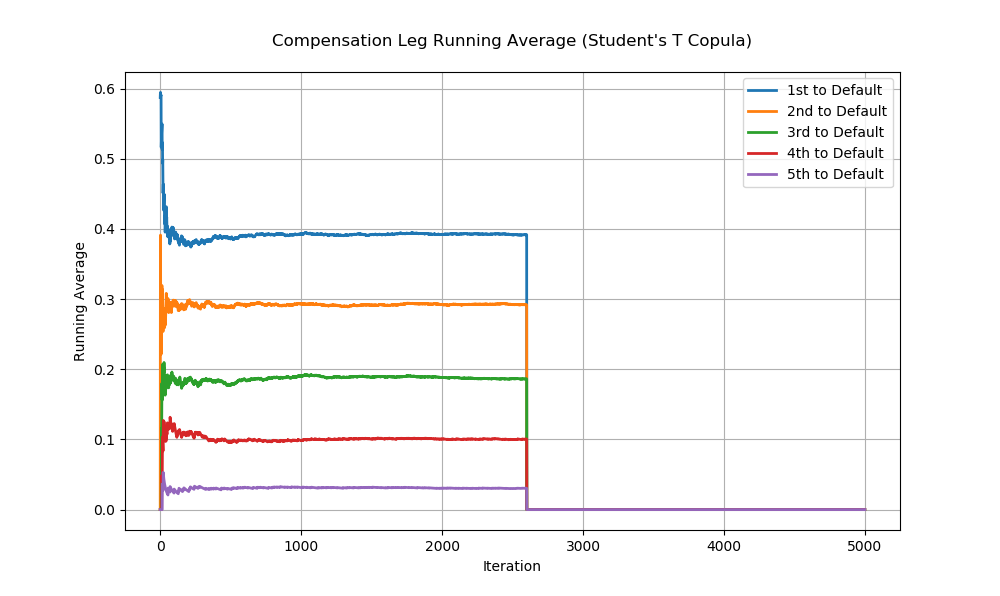
\includegraphics[width=15cm]{Compensation_Leg_Running_Average_(Student's_T_Copula).png}
		\caption{Running Average of Compensation Leg for the Student's T Copula} 
		\label{Compensation_Leg_Running_Average_(Student's_T_Copula)}
	\end{center}
\end{figure}

\begin{figure}[H]
	\begin{center}
		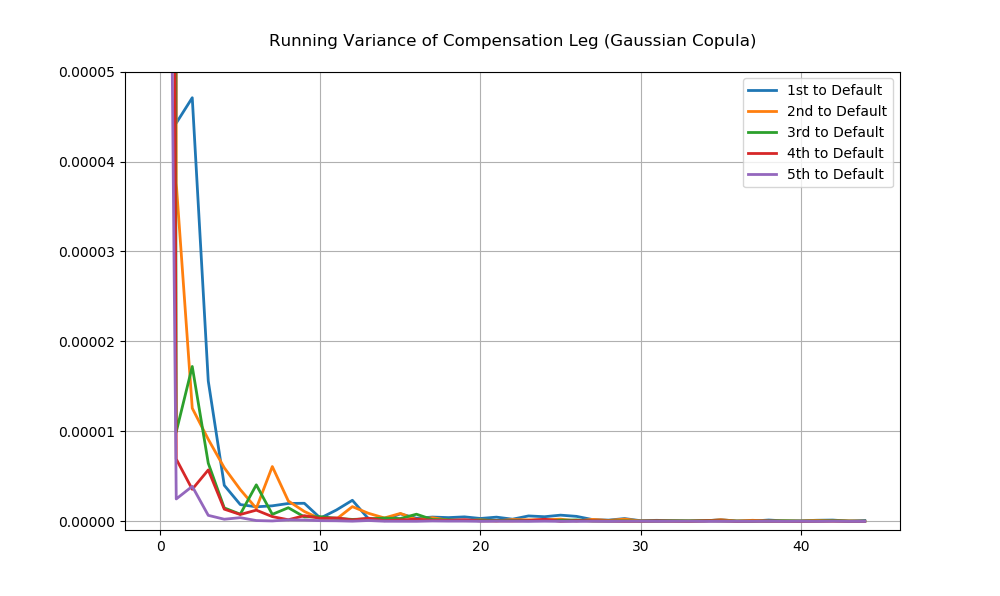
\includegraphics[width=15cm]{Running_Variance_of_Compensation_Leg_(Gaussian_Copula).png}
		\caption{Running Variance of Compensation Leg for the Gaussian Copula} 
		\label{Running_Variance_of_Compensation_Leg_(Gaussian_Copula)}
	\end{center}
\end{figure}

\begin{figure}[H]
	\begin{center}
		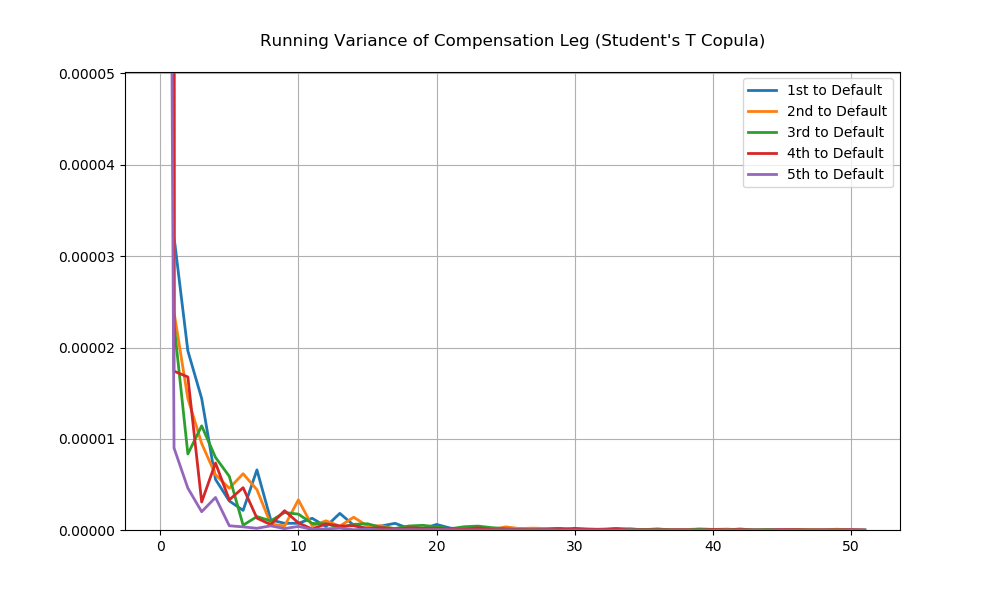
\includegraphics[width=15cm]{Running_Variance_of_Compensation_Leg_(Student's_T_Copula).png}
		\caption{Running Variance of Compensation Leg for the Student's T Copula} 
		\label{Running_Variance_of_Compensation_Leg_(Student's_T_Copula)}
	\end{center}
\end{figure}

\begin{figure}[H]
	\begin{center}
		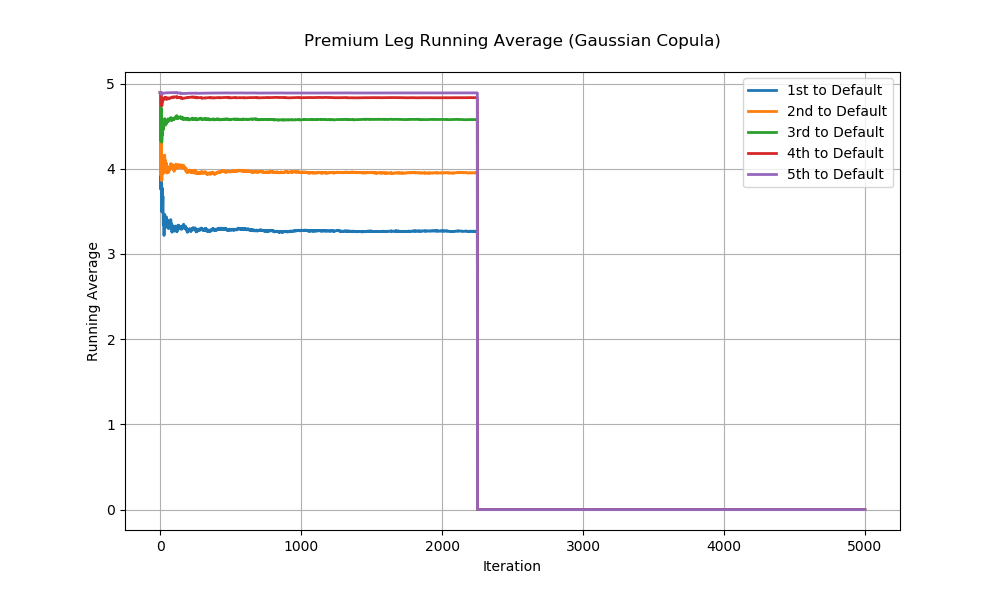
\includegraphics[width=15cm]{Premium_Leg_Running_Average_(Gaussian_Copula).png}
		\caption{Running Average of Premium Leg for the Gaussian Copula} 
		\label{Premium_Leg_Running_Average_(Gaussian_Copula)}
	\end{center}
\end{figure}

\begin{figure}[H]
	\begin{center}
		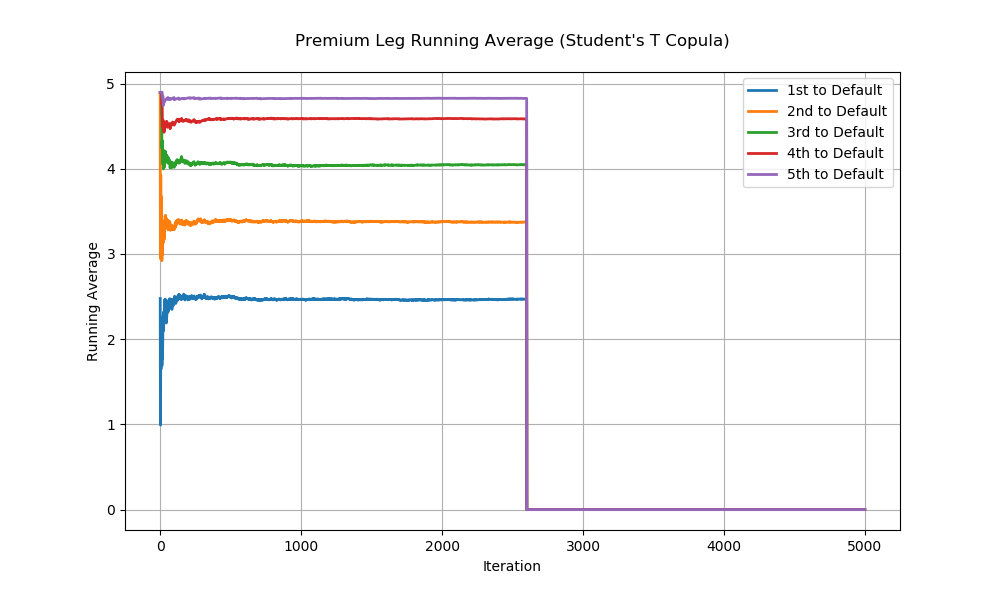
\includegraphics[width=15cm]{Premium_Leg_Running_Average_(Student's_T_Copula).png}
		\caption{Running Average of Premium Leg for the Student's T Copula} 
		\label{Premium_Leg_Running_Average_(Student's_T_Copula)}
	\end{center}
\end{figure}

\begin{figure}[H]
	\begin{center}
		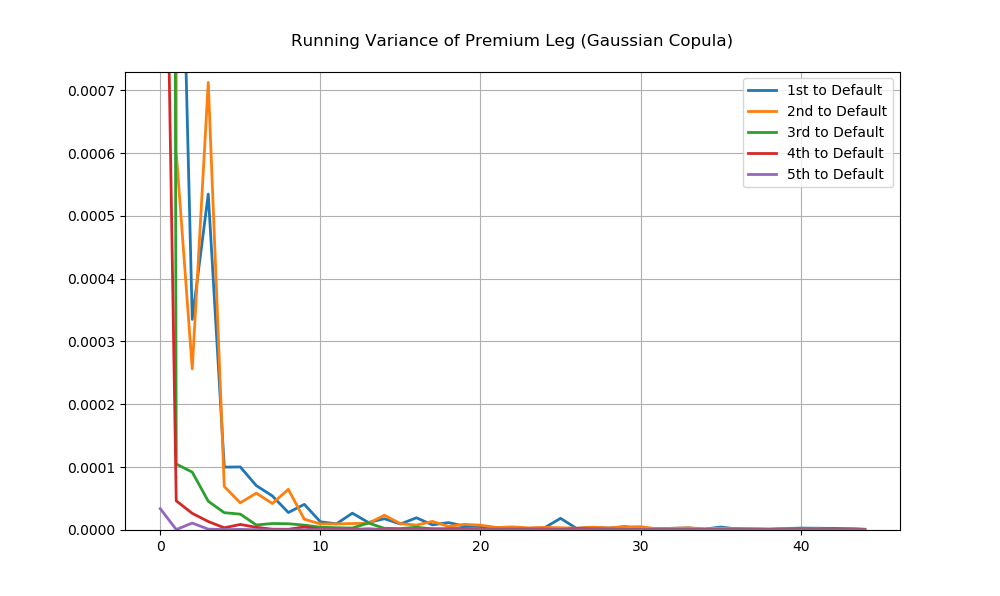
\includegraphics[width=15cm]{Running_Variance_of_Premium_Leg_(Gaussian_Copula).png}
		\caption{Running Variance of Premium Leg for the Gaussian Copula} 
		\label{Running_Variance_of_Premium_Leg_(Gaussian_Copula)}
	\end{center}
\end{figure}

\begin{figure}[H]
	\begin{center}
		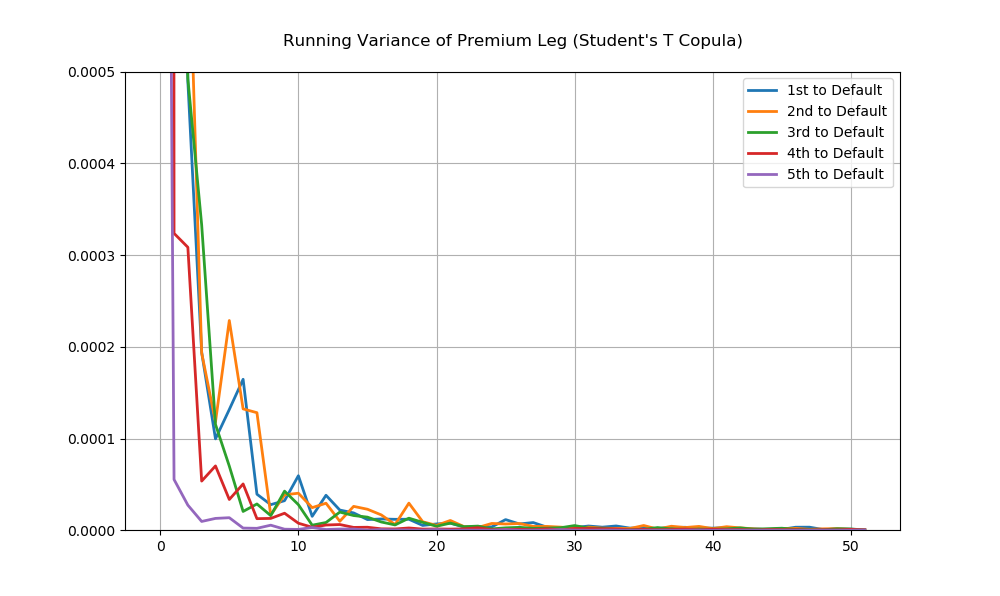
\includegraphics[width=15cm]{Running_Variance_of_Premium_Leg_(Student's_T_Copula).png}
		\caption{Running Variance of Premium Leg for the Student's T Copula} 
		\label{Running_Variance_of_Premium_Leg_(Student's_T_Copula)}
	\end{center}
\end{figure}


The simulation outputs the following estimates of fair spreads for the $1^{st}$ to the $5^{th}$ to default instruments respectively for both the Gaussian and the Student's T assumption.

\begin{center}
	\begin{tabular}{|l|l|l|l|l|c|c|c|c|c|}
		\hline
		\textbf{} & \textbf{$1^{st}$} & \textbf{$2^{nd}$} & \textbf{$3^{rd}$} & \textbf{$4^{th}$} & \textbf{$5^{th}$}\\\hhline{|=|=|=|=|=|=|}
		\textbf{Gaussian} & 0.101567982756 & 0.0501498757102 & 0.0274859057615 & 0.00812602603563 & 0.00146327454895\\
		\textbf{Student's T} & 0.15864249598 & 0.0865140811474 & 0.046047608693 & 0.021924513683 & 0.00629194399778\\
		\hline
	\end{tabular}
\end{center}


%Decide if these values are acceptable.
I compare these values with the market spreads on 5 year CDS contracts for the reference names as it would make intuitive sense to observe that the smallest observed market spread is greater than or equal to the $5^{th}$-to-default fair basket spread seeing as the $5^{th}$-to-default basket must by definition default after or at the same time as the default of the reference name with the smallest spread. Conversely, one should see that the largest observed marked spread is less than or equal to the $1^{st}$-to-default fair basket spread seeing as the $1^{st}$-to-default basket must by definition default before or at the same time as the default of the reference name with the greatest spread. So comparing these rates with the 5 year CDS contracts, I notice that this condition is met.\\

I next compare the differences in the fair spreads for the different $k^{th}$-to-default baskets due to the choice of underlying default distribution.\\

%plot of both sets of spreads on same plot

I observe that the spread of the baskets that sampled from a Student's T distribution is always greater than the Gaussian comparison. The earlier simulated defaults of the Student's T copula reflect the copula's heavier tails which can be seen in Figure \ref{T_Copula_3_vs_T_Copula_4} in comparison to Figure \ref{Gaussian_Copula_1_vs_Gaussian_Copula_2}.


\chapter{Model Validation}

\section{Re-Pricing with Fair Spread to compare Premiums and Compensation}
In this section, I use the fair spread calculated above and perform another simulation, this time using the fair spread. The goal is to check that the mean value of the compensation legs should be roughly equal to the mean value of the premium legs, otherwise the spread is not fair.

\section{Comparison of spreads by instrument}
If one compares the $k^{th}$ to default spread with the $(k-1)^{th}$ spread, the latter should be less because there is by definition a lower probability that the $k^{th}$ reference name defaults before the maturity of the CDS. Stated explicitly, this is because the $(k-1)^{th}$ reference name must, by definition, have already defaulted. This constraint is satisfied according to resulting spreads above.

\section{Model Sensitivity to Recovery Rates}
One would expect to notice an inverse relationship between the recovery rate the fair spread of the $k^{th}$ to default basket. 

I decide to try a range of Recovery rates where the recovery rate is equivalent across reference names. \\

Under the Gaussian model, I observe the following relationship which confirms the expected relationship for the fair spreads:

\begin{figure}[H]
	\begin{center}
		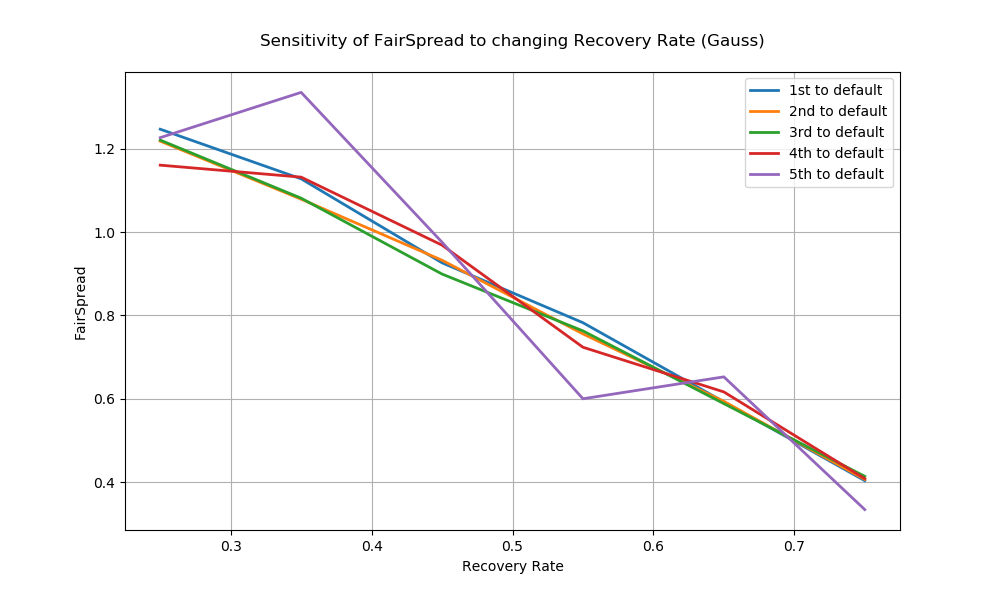
\includegraphics[width=15cm]{Sensitivity_of_FairSpread_to_changing_Recovery_Rate_(Gauss).png}
		\caption{Sensitivity of fair spread to recovery rate (Gaussian)} 
		\label{Sensitivity_of_FairSpread_to_changing_Recovery_Rate_(Gauss)}
	\end{center}
\end{figure}

For the Student's T model, I also observe the same relationship which again confirms the expected relationship for the fair spreads: 

\begin{figure}[H]
	\begin{center}
		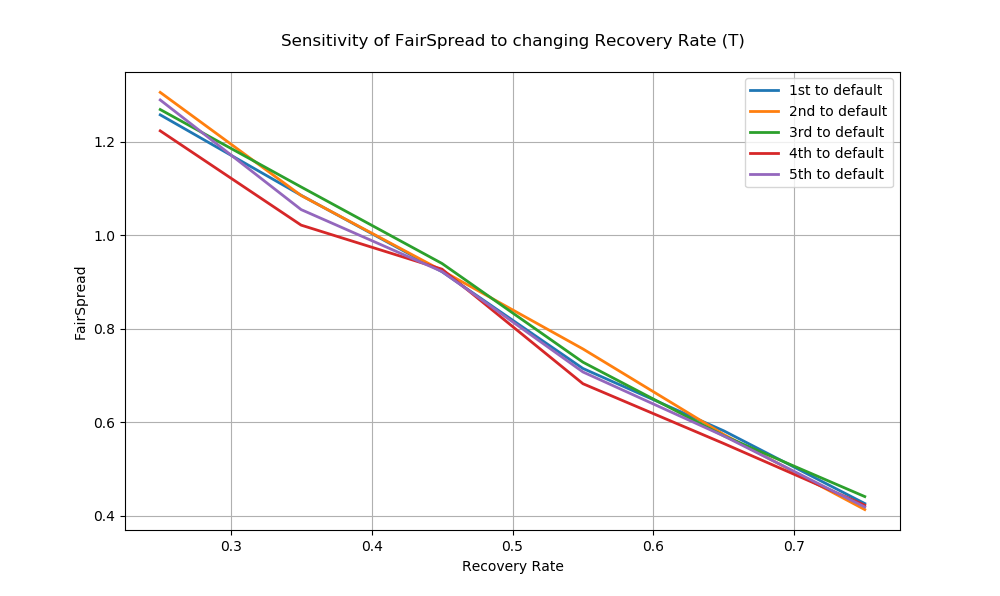
\includegraphics[width=15cm]{Sensitivity_of_FairSpread_to_changing_Recovery_Rate_(T).png}
		\caption{Sensitivity of fair spread to recovery rate (Student's T)} 
		\label{Sensitivity_of_FairSpread_to_changing_Recovery_Rate_(T)}
	\end{center}
\end{figure}

\section{Model Sensitivity to Individual Reference Names}

In this section, I consider how sensitive each of the k$^{th}$ to default instruments is to the spread of each individual reference name. I increase the credit spreads for one to 5 year tenors of one reference name at a time and observe the difference in the spreads for each of the k$^{th}$ to default instruments. It is assumed and expected that the fair spread for each of the instruments increases when the underlying credit spreads of one of the baskets constituents are increased.

To visualise the increase in spread with respect to increasing the market observed spreads of each individual reference name, I display a barchart which shows the increase in spread for all instruments on the same bar (1$^{st}$ to 5$^{th}$ upwards) with respect to the increase in spread of a reference name.

\begin{figure}[H]
	\begin{center}
		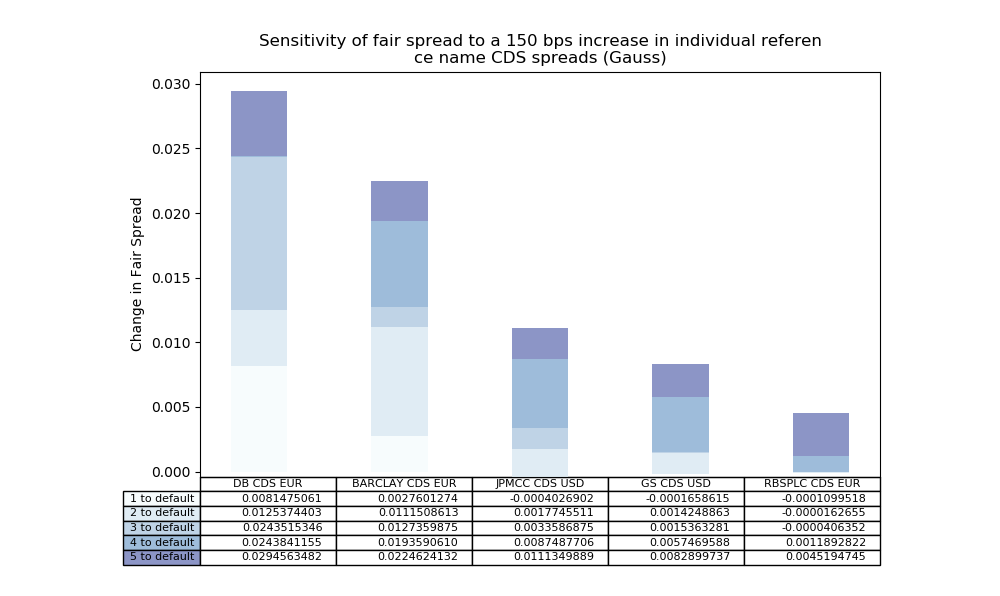
\includegraphics[width=15cm]{Sensitivity_of_fair_spread_to_a_150_bps_increase_in_individual_reference_name_CDS_spreads_(Gauss).png}
		\caption{Sensitivity of fair spread to Credit Spread Deltas (Gauss)} 
		\label{Sensitivity_of_fair_spread_to_a_150_bps_increase_in_individual_reference_name_CDS_spreads._(Gauss)}
	\end{center}
\end{figure}


\begin{figure}[H]
	\begin{center}
		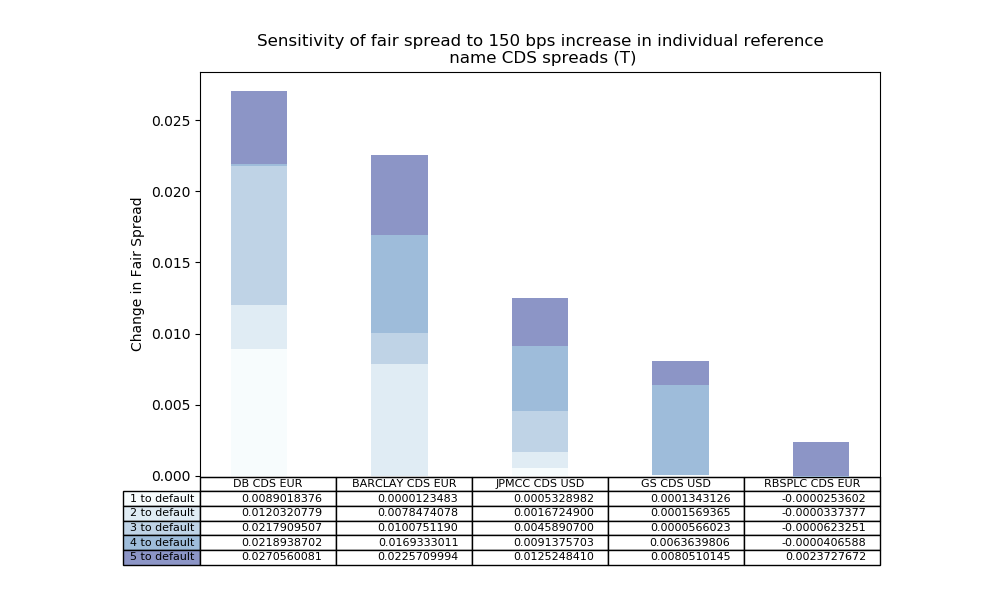
\includegraphics[width=15cm]{Sensitivity_of_fair_spread_to_150_bps_increase_in_individual_reference_name_CDS_spreads_(T).png}
		\caption{Sensitivity of fair spread to Credit Spread Deltas (Student's T)} 
		\label{Sensitivity_of_fair_spread_to_150_bps_increase_in_individual_reference_name_CDS_spreads._(T)}
	\end{center}
\end{figure}

From both barcharts, I observe the following:
\begin{enumerate}
	\item Hi
\end{enumerate}


\section{Model Sensitivity to Default Correlations}

In this section, I force arbitrary changes / values on the default correlations for both:
\begin{itemize}
	\item Individual pairwise default dependencies between reference names.
	\item All the reference names in the basket together. 
\end{itemize}

Below, I observe the sensitivity of the fair spreads to the Correlation matrix and therefore the generated copulas.

\subsection{Gaussian Copula}

\begin{figure}[H]
	\begin{center}
		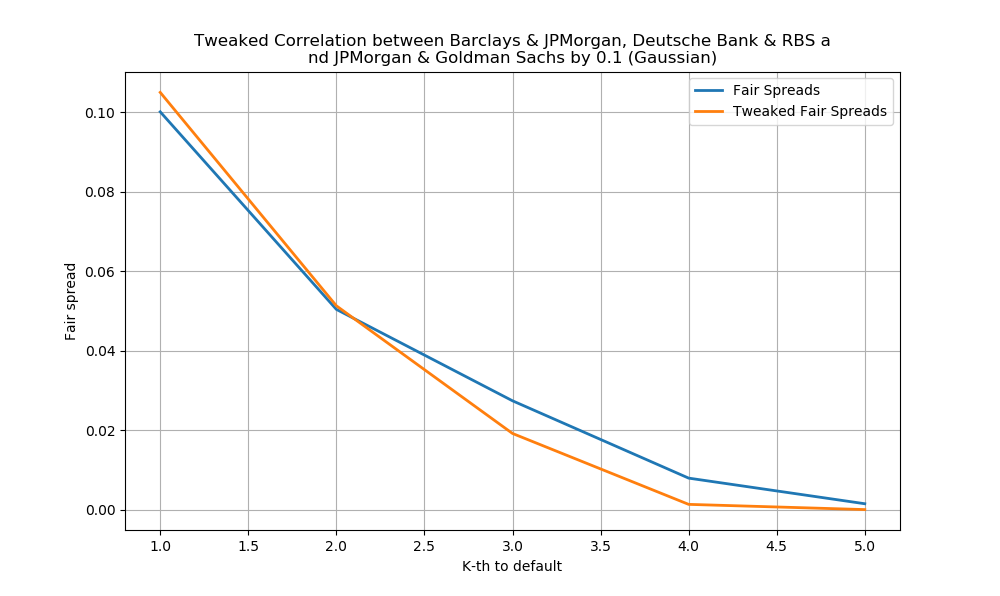
\includegraphics[width=15cm]{Tweaked_Correlation_between_Barclays_&_JPMorgan,_Deutsche_Bank_&_RBS_and_JPMorgan_&_Goldman_Sachs_by_0,1_(Gaussian).png}
		\caption{Sensitivity of fair spread to tweaking Correlation for (Barc,JPM), (DB,RBS) \& (JPM,GS) by 0.1} 
		\label{Tweaked_Correlation_between_Barclays_&_JPMorgan,_Deutsche_Bank_&_RBS_and_JPMorgan_&_Goldman_Sachs_by_0.1_(Gaussian)}
	\end{center}
\end{figure}

\begin{figure}[H]
	\begin{center}
		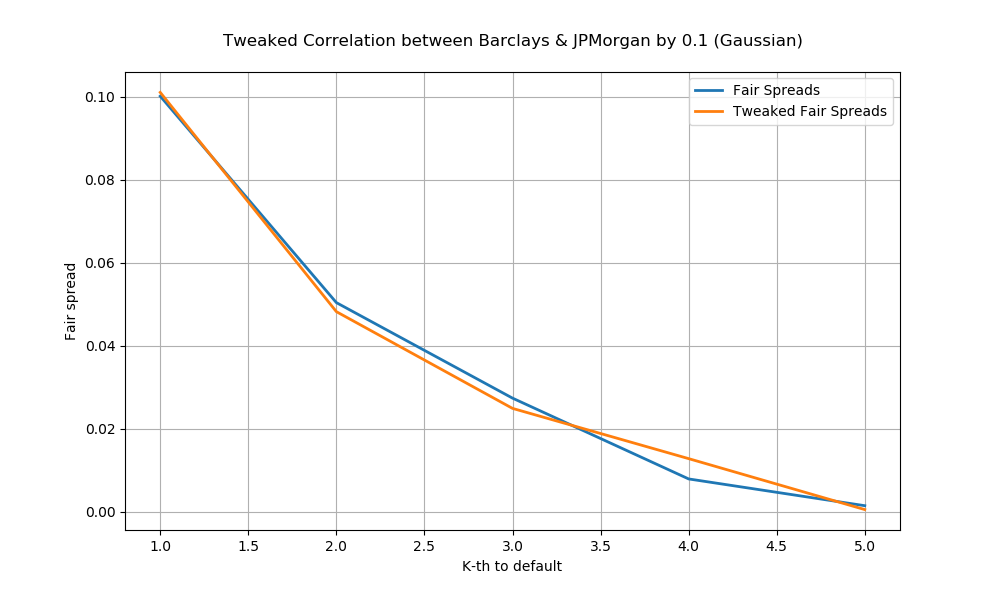
\includegraphics[width=15cm]{Tweaked_Correlation_between_Barclays_&_JPMorgan_by_0,1_(Gaussian).png}
		\caption{Sensitivity of fair spread to tweaking Correlation for (Barc,JPM) by 0.1} 
		\label{Tweaked_Correlation_between_Barclays_&_JPMorgan_by_0.1_(Gaussian)}
	\end{center}
\end{figure}

\begin{figure}[H]
	\begin{center}
		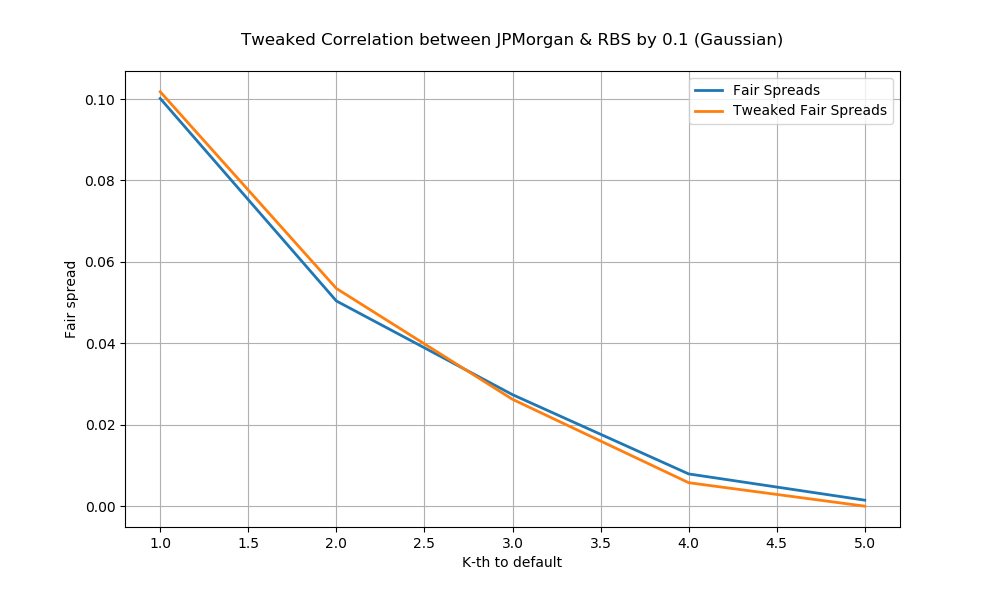
\includegraphics[width=15cm]{Tweaked_Correlation_between_JPMorgan_&_RBS_by_0,1_(Gaussian).png}
		\caption{Sensitivity of fair spread to tweaking Correlation for (JPM,RBS) by 0.1} 
		\label{Tweaked_Correlation_between_JPMorgan_&_RBS_by_0.1_(Gaussian)}
	\end{center}
\end{figure}

\begin{figure}[H]
	\begin{center}
		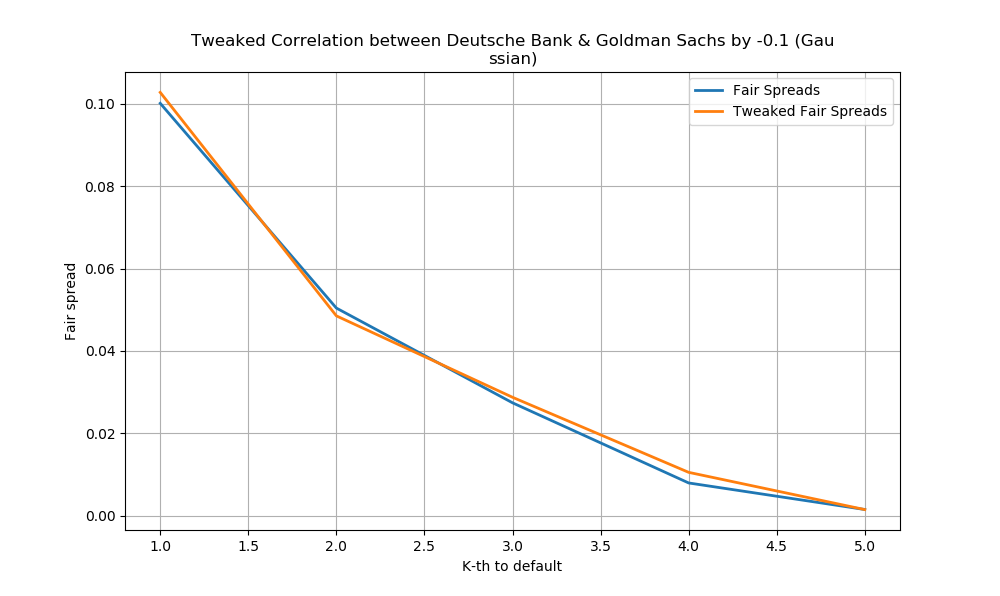
\includegraphics[width=15cm]{Tweaked_Correlation_between_Deutsche_Bank_&_Goldman_Sachs_by_-0,1_(Gaussian).png}
		\caption{Sensitivity of fair spread to tweaking Correlation for (DB,GS) by -0.1} 
		\label{Tweaked_Correlation_between_Deutsche_Bank_&_Goldman_Sachs_by_-0.1_(Gaussian)}
	\end{center}
\end{figure}


\subsection{Student's T Copula}

\begin{figure}[H]
	\begin{center}
		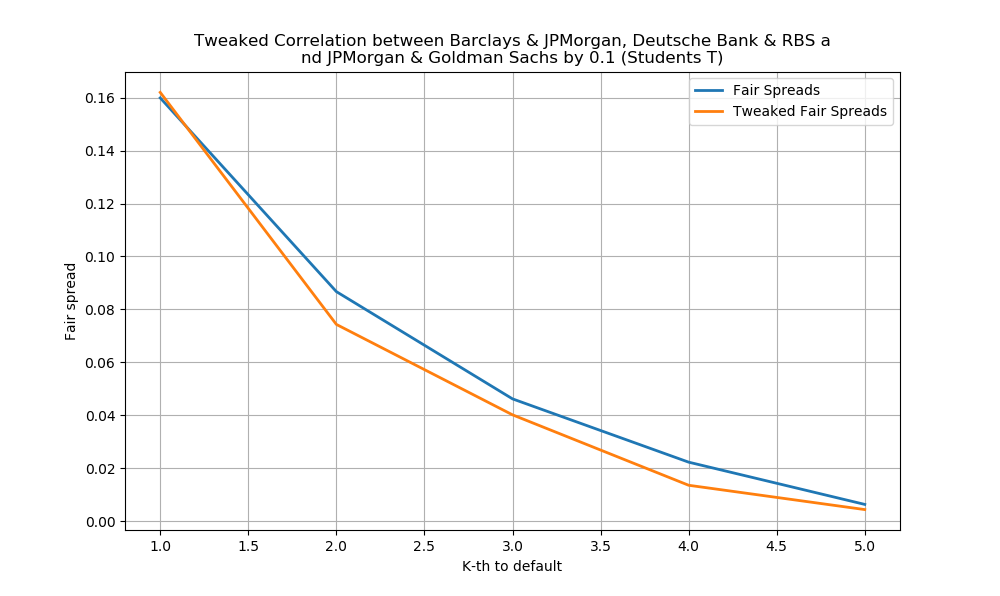
\includegraphics[width=15cm]{Tweaked_Correlation_between_Barclays_&_JPMorgan,_Deutsche_Bank_&_RBS_and_JPMorgan_&_Goldman_Sachs_by_0,1_(Students_T).png}
		\caption{Sensitivity of fair spread to tweaking Correlation for (Barc,JPM), (DB,RBS) \& (JPM,GS) by 0.1} 
		\label{Tweaked_Correlation_between_Barclays_&_JPMorgan,_Deutsche_Bank_&_RBS_and_JPMorgan_&_Goldman_Sachs_by_0.1_(Students_T)}
	\end{center}
\end{figure}

\begin{figure}[H]
	\begin{center}
		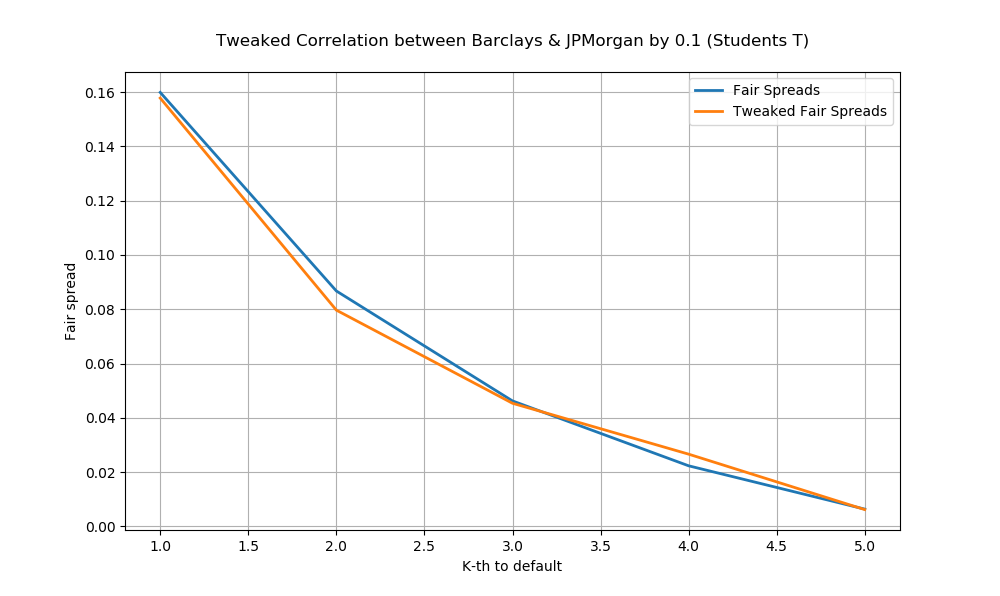
\includegraphics[width=15cm]{Tweaked_Correlation_between_Barclays_&_JPMorgan_by_0,1_(Students_T).png}
		\caption{Sensitivity of fair spread to tweaking Correlation for (Barc,JPM) by 0.1} 
		\label{Tweaked_Correlation_between_Barclays_&_JPMorgan_by_0.1_(Students_T)}
	\end{center}
\end{figure}

\begin{figure}[H]
	\begin{center}
		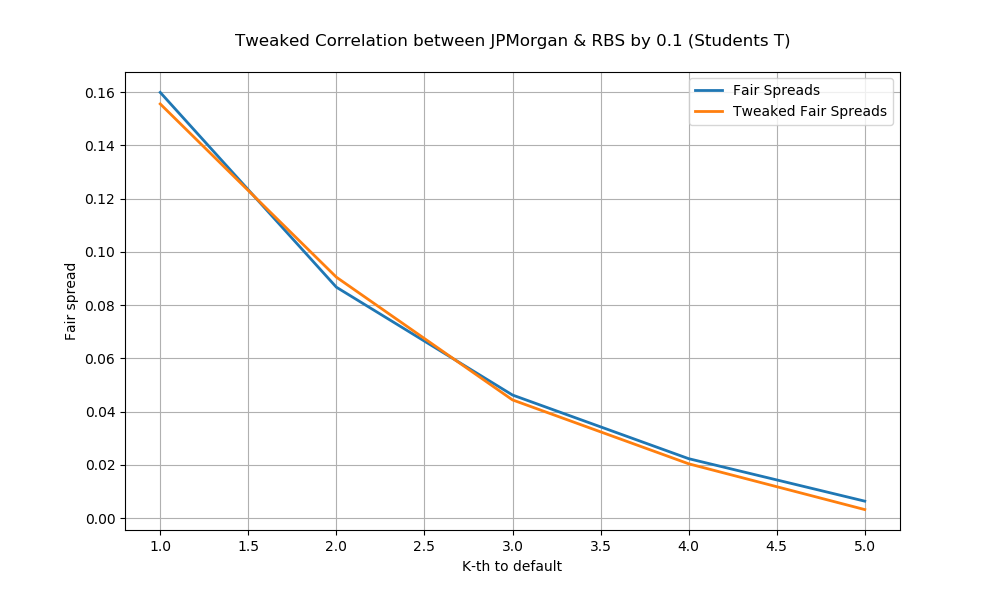
\includegraphics[width=15cm]{Tweaked_Correlation_between_JPMorgan_&_RBS_by_0,1_(Students_T).png}
		\caption{Sensitivity of fair spread to tweaking Correlation for (JPM,RBS) by 0.1} 
		\label{Tweaked_Correlation_between_JPMorgan_&_RBS_by_0.1_(Students_T)}
	\end{center}
\end{figure}

\begin{figure}[H]
	\begin{center}
		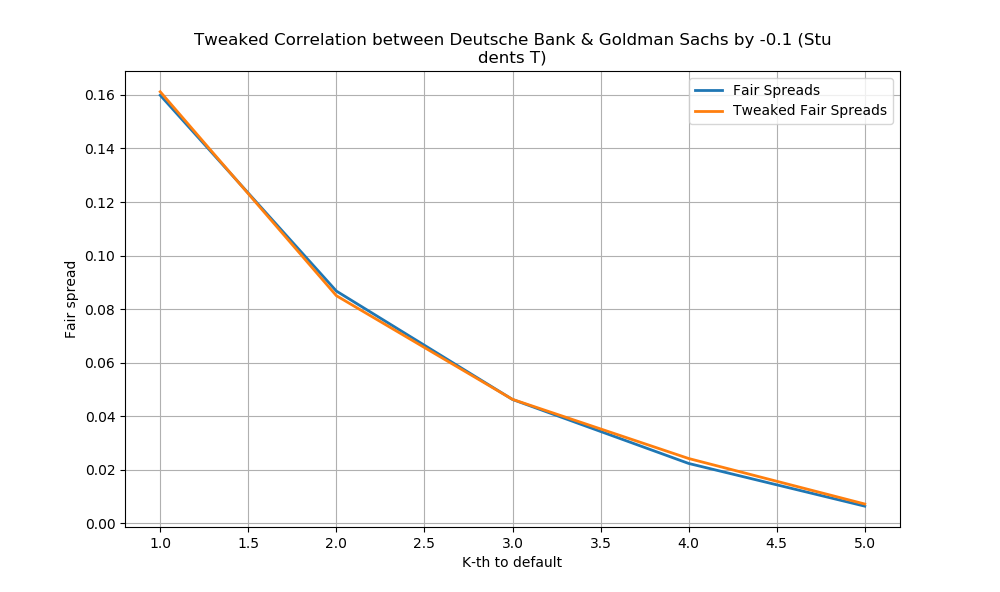
\includegraphics[width=15cm]{Tweaked_Correlation_between_Deutsche_Bank_&_Goldman_Sachs_by_-0,1_(Students_T)}
		\caption{Sensitivity of fair spread to tweaking Correlation for (DB,GS) by -0.1} 
		\label{Tweaked_Correlation_between_Deutsche_Bank_&_Goldman_Sachs_by_-0.1_(Students_T)}
	\end{center}
\end{figure}

\subsection*{Conclusion}

If I consider an individual Asian Call Option, then the difference in expected value between the different specification of contract doesn't differ overly much. However, I notice that the combination of Floating Geometric and Fixed Arithmetic have slightly higher values than Floating Arithmetic and Fixed Geometric. The opposite scenario is observed for the Asian Put Option. This is because the Average is larger when calculated using the Arithmetic approach over the geometric approach. This penalises the payoff of the Asian Call Option with floating strike and rewards the payoff of the Asian Call Option with fixed strike.\newline
\\
The option is priced at the money, hence the expected value of the put is only marginally smaller than the expected value of the call. This makes sense from the drift of the underlying that rewards the call and penalises the put.\newline
\\
The introduction of Jumps in the underlying stock substantially increases the Expected Payoff of the Asian Call Option and marginally increases the value of the Asian Put Option. If we consider the jumps to be similar to an increase in the volatility of the stock, then despite the interest rate adjustment paramter $r_j$, the increased spread of paths causes the possible payoff to increase to higher levels. Whereas in the opposite direction, both the payoff and underlying stock are bounded below by zero. This effect is observed  by comparing the histograms given with and without jumps. I notice, that the probabilty of having a discounted payoff of 0 is lower when jumps are introduced.

\subsection*{References}

\begin{itemize}
  \item \textbf{CQF Intro to Python Lecture given by Dr. Yves J. Hilpisch with notes\\at: https://gist.github.com/yhilpisch/e2af84bc2ff1cab88d6be019459f5672.}

  \item \textbf{CQF Lecture Notes}
\end{itemize}



\end{document}